%%%%%%%%%%%%%%%%%%%%%%%%%%%%%%%%%%%%%%%%%%%%%%%%%%%%%%%%%
%       KAPITOLA 1 - Úvod
%%%%%%%%%%%%%%%%%%%%%%%%%%%%%%%%%%%%%%%%%%%%%%%%%%%%%%%%%
\chapter{Úvod}
\label{kapitola:uvod}
Neuronové sítě (anglicky neural networks) mají v~dnešním světě mnoho využití. Jelikož se jedná o~jednu z~aplikací umělé inteligence (anglicky artificial intelligence), lze neuronové sítě použít například k~rozpoznávání řeči, zpracování přirozeného jazyka či k~detekci obličejů.
Tyto činnosti jsou pro běžného člověka poměrně snadné, avšak pro počítače znamenají relativně náročnou činnost.

Lidé jsou schopni velmi dobře rozeznat obličeje jiných lidí, bez ohledu na světelné podmínky, úhel natočení či částečné zakrytí tváře. Počítačové algoritmy a neuronové sítě zaměřující se na detekci obličejů v~těchto neideálních podmínkách musí být těmto jevů přizpůsobeny.

Aby byly počítače schopné tyto akce vykonávat v~rozumném čase (případně v~reálném čase), je potřeba, aby neuronové sítě byly dostatečně rychlé. Zrychlení neuronové sítě lze dosáhnout buď optimalizací kódu, vylepšením procesu trénování neuronové sítě nebo také využitím speciálních hardwarových zařízení. 

Tato práce se zabývá problematikou výše zmíněných fenoménů, konkrétně optimalizací a zrychlením neuronových sítí pro detekci obličejů v~neoptimálních světelných podmínkách. Z~oblasti neuronových sítí byly použity konvoluční neuronové sítě, k~jejichž trénování je využito jak dat z~běžných datasetů tváří, tak dat ze specializovaných datasetů obličejů a~osob ve špatném osvětlení. 

O~akceleraci neuronové sítě se stará zařízení Intel Neural Compute Stick 2 (NCS2) s~knihovnou OpenVINO. V~práci jsou také zmíněny dostupné komerční a~nekomerční systémy a~řešení pro detekci obličejů.

V~rámci kapitoly \ref{kapitola:detekce_obliceje} je popsána problematika detekce obličeje v~reálných podmínkách, včetně problémů, které detekci ztěžují či přímo znemožňují. Tato část také popisuje klasické přístupy k~detekci obličejů jako jsou algoritmy Viola--Jones nebo Local Binary Patterns.

Kapitola \ref{kapitola:neuronove_site} se věnuje neuronovým sítím jak obecně (perceptron, aktivační funkce, učení), tak konkrétně konvolučním neuronovým sítím. Dále jsou v~kapitole popsány datasety pro učení neuronových sítí a existující řešení detekce obličeje založené na neuronových sítích (YOLO, MTCNN, SSD), včetně jejich porovnání a porovnání algoritmů zaměřených na detekci ve špatných světelných podmínkách.

Popis používaných řešení a systémů k~detekci a popis akcelerace detekčních algoritmů tvoří obsah kapitoly \ref{kapitola:kamery_a_systemy}. Konkrétně je zde popsáno zařízení NCS2.



%%%%%%%%%%%%%%%%%%%%%%%%%%%%%%%%%%%%%%%%%%%%%%%%%%%%%%%%%
%       KAPITOLA 2 - Detekce obličejů
%%%%%%%%%%%%%%%%%%%%%%%%%%%%%%%%%%%%%%%%%%%%%%%%%%%%%%%%%
\chapter{Detekce obličeje v~reálných podmínkách}
\label{kapitola:detekce_obliceje}
Detekce obličeje (anglicky face detection) \cite{fdReview, frReview} je technologie, která umožňuje v~digitálním obrázku lokalizovat lidský obličej. Detekce obličeje patří do skupiny technologií HCI (Human--Computer interaction).
Detekovat obličej je poměrně jednoduchý úkol pro lidi, ale zároveň se jedná o~relativně náročný úkol pro počítače.
Detekce obličeje je výchozím bodem pro další algoritmy analyzující lidský obličej, jako je například (v~závorce za pojmem následuje anglický výraz):
\begin{itemize}
  \item rozpoznávání obličeje (face recognition),
  \item zarovnání obličeje (face alignment),
  \item autentizace pomocí obličeje (face verification/authentication),
  \item sledování pohybu hlavy (head pose tracking),
  \item určování věku nebo pohlaví (age/gender recognition),
  \item[] a mnoho dalších. 
\end{itemize}

Samotná detekce obličeje se v~realném prostředí využívá například v~oblasti fotografování (automatické ostření na tvář), marketingu (zjišťování zájmu zákazníku o~produkty podle počtu výskytu obličejů) nebo bezpečnosti (bezpečnostní kamery a systémy).

Následující podkapitoly se zabývají principem fungování detekce obličeje v~reálných podmínkách a problémy a omezeními, které se v~běžném světě vyskytují a detekce by si s~nimi měla umět poradit (špatné světelné podmínky, příliš členité pozadí, přílišný počet obličejů v~obrázku, barva kůže, nízké rozlišení atd.). Na konci této kapitoly se nachází popis algoritmů a detektorů, které k~detekci přímým způsobem nepoužívají neuronové sítě.

\begin{figure}[H]
  \begin{center}
      \scalebox{0.31}{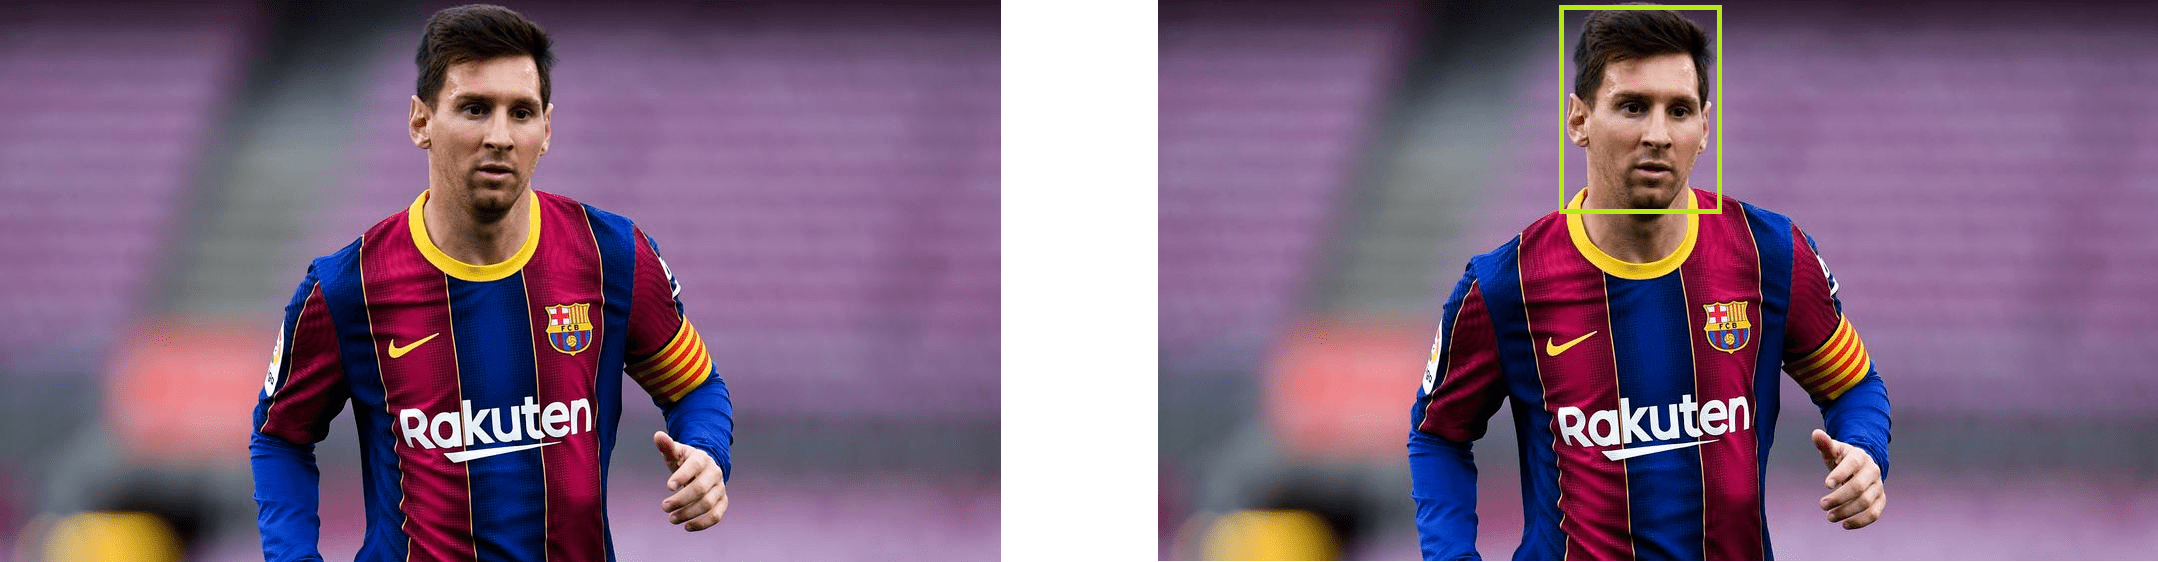
\includegraphics{obrazky-figures/fdexample.png}}
  \label{fdexample}
  \caption{Příklad detekce obličeje}
  \end{center}
\end{figure}

\section{Detekce obličeje}
Způsoby detekce obličeje lze rozdělit do několika skupin, vědecké práce na toto téma se liší a nelze jasně říci zda to či ono dělení je jediné korektní.

Dle \cite{fdReview} existují 2 různé přístupy k~hledání tváří v~obrázcích, a to \textbf{přístup založený na vlastnostech} (anglicky feature based approach) a \textbf{přístup založený na obrázku} (anglicky image based approach). 
\textbf{Přístup založený na vlastnostech} nepoužívá přímo k~detekci obličeje neuronové sítě. Využívá vlastností obličeje jako takového (rysy, pozice očí, uší, obočí, barva kůže\dots). Efektivita tohoto přístupu se snižuje s~výskyty problémů popsaných v~sekci \ref{sekce:problemy}, protože může docházet například k~zakrytí nebo špatné viditelnosti některých vlastností obličeje.

Naproti tomu \textbf{obrazový přístup} uplatňuje schopnosti neuronových sítí a umělé inteligence k~natrénování modelu neuronové sítě a následné přímé detekci pomocí tohoto modelu. 

Podle \cite{feature-based-fd-review} lze rozdělit metody detekce obličeje do 4 základních kategorií (viz obrázek \ref{fddeleni}) a 2 zvláštních kategorií (Haarovy vlastnosti a umělá inteligence).
\begin{figure}[H]
  \begin{center}
      \scalebox{0.9}{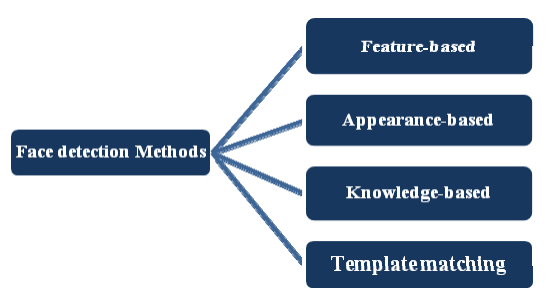
\includegraphics{obrazky-figures/fddeleni.png}}
  \label{fddeleni}
  \caption{Dělení metod detekce obličeje dle \cite{feature-based-fd-review}}
  \end{center}
\end{figure}

\textbf{Feature-based methods} (metody založené na vlastnostech) opět pracují s~vlastnostmi obličeje. Vyhledávají v~obraze rysy obličeje. Detekci může výrazně ztížit či znemožnit neviditelnost některých rysů. Výhodou těchto metod je rychlost v~porovnání s~ostatními metodami.

\textbf{Appearance-based methods} (metody založené na vzhledu/obrázku) využívají klasifikace vlastností tváře do 2 tříd v~podobrázku celého obrázku. Klasifikátory podle nichž se daná metoda rozhoduje, zda se jedná o~tvář či nikoli, mají různé váhy, metoda postupuje od slabých klasifikátorů k~silnějším.

Metody založené na znalostech (\textbf{Knowledge-based mathods}) se uplatňují při detekci obličeje v~obrázku s~členitým/komplexním pozadím. Znalosti, které k~detekci pomáhají jsou například: obličej má 2 uši, jeden nos, jedny ústa nebo známé vzdálenosti mezi jednotlivými rysy obličeje.

\textbf{Templatematching} (šablonování, maskování) aplikuje na obrázek předem danou ma-sku obličeje a snaží se detekovat obličej pomocí postupného maskování. Tato metoda je snadná na implementaci, jejím nedostatkem je však závislost na přímém pohledu tváře na obrázku.

Haarovými vlastnostmi a neuronovými sítěmi se zabývají sekce \ref{sekce:viola_jones}, respektive \ref{sekce:NS}.

\section{Problémy a omezení}
\label{sekce:problemy}
Algoritmy pro detekci obličejů čelí několika výzvám a omezením spojených s~ne vždy perfektním zobrazením obličeje v~obrázku. Lidské obličeje na fotografiích a obrázcích mohou být částečně zakryté (např. sluneční brýle), fotografie mohou být pořízené za nevhodných světelných podmínek (např. zastínění části tváře) nebo mohou obrázky nabývat nedostatečné kvality (nízké rozlišení).

Jelikož tedy vstupní obrázek detekce obličeje nemusí být vždy ideální, nemusí být obličej vždy správně detekován.
V~této sekci jsou popsány některé problémy \cite{feature-based-fd-review, fdReview}, které mohou bránit v~úspěšné detekci. Minimalizace dopadu těchto jevů na detekci je klíčem k~navýšení uspěšnosti detekce. Mezi problémy a omezení (viz obrázek \ref{fdproblems}) pro detekci patří pozice hlavy, zakrytí části/částí obličeje, špatně osvětlená scéna nebo výraz tváře.

\begin{figure}[H]
  \begin{center}
      \scalebox{0.5}{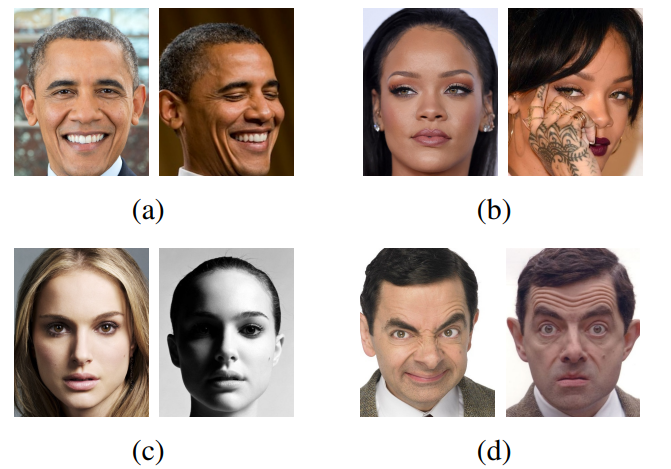
\includegraphics{obrazky-figures/fdproblems.png}}
  \label{fdproblems}
  \caption{Vybráné problémy při detekci obličejů \cite{frReview}. (a) Pozice hlavy; (b)~Zakrytí části obličeje; (c) Špatné světelné podmínky; (d) Výraz tváře}
  \end{center}
\end{figure}

\subsection*{Pozice hlavy}
Hlava může být na fotografii různě natočena, takže obličej nemusí být zachycen v~přímém pohledu do kamery, ale může být zaznamenán z~profilu nebo ze šikma (poloprofil) jako na obrázku \ref{fdproblems} část (a).

\subsection*{Zakrytí části obličeje}
Výsledek detekce může být ovlivněn i zakrytím části obličeje (rukou, brýlemi, vlasy, šátkem apod.).

\subsection*{Výraz tváře}
Výraz lidského obličeje mohou ovlivnit emoce a nálady. Detektor \cite{emotionDetector} zabývající se detekcí a rozpoznáváním emocí dosahuje přesnosti 96 \%.

\subsection*{Orientace obrázku}
Problémem pro detekci může být různá orientace obrázku (vzhůru nohama, zrcadlově otočený, natočený do strany apod.). Na obrázek je tak nutno aplikovat některé tranformační operace pro zarovnání.


\subsection*{Nedostatečně výkonná detekce}
Velmi důležitým faktorem při detekci obličejů, zvláště v~real-timových aplikacích, je rychlost detekce. Pokud má algoritmu vysokou přesnost, ale je příliš pomalý pro vybranou aplikaci, stává se nepoužitelným. Akcelerací detekčních algoritmů se mj. zabývá i tato práce.

\subsection*{Příliš členité pozadí} 
Pokud se v~o~brázku nachází příliš mnoho objektů, může dojít ke snížení přesnosti a rychlosti detekce.

\subsection*{Přílišný počet obličejů v~obrázku}
Výskyt velkého počtu obličejů v~jednom obrázku, často překrývajících se, může představovat výzvu pro detekční algoritmus. 

\subsection*{Nízké rozlišení}
Obrázky a fotografie s~nízkým rozlišením nemusejí obsahovat dostatek informace nutné ke správnemu detekování tváře.

\subsection*{Špatné světelné podmínky}
Na detekci mohou mít vliv světelné podmínky panující při pořizování zkoumané fotografie či videa. Aspekty jež světlo ovlivňuje jsou mj. jas, kontrast, barvy, stíny, ostrost. Tato práce se zabývá detekcí obličejů v~záznamech, v~nichž některý z~těchto faktorů omezuje detekci.


\begin{figure}[H]
  \begin{center}
      \scalebox{0.8}{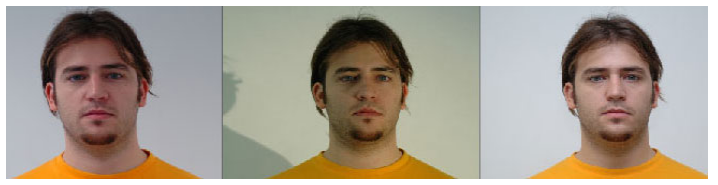
\includegraphics{obrazky-figures/illuminationexample.png}}
  \label{illuminationexample}
  \caption{Příklad stejného obličeje vyfoceného při různých světelných podmínkách \cite{feature-based-fd-review}}
  \end{center}
\end{figure}

\section{Algoritmy detekce obličeje}
\label{sekce:detektory_bez_neuronovych_siti}
Existuje několik různých přístupů k~detekci obličeje. Tato sekce se zaměřuje na detekci s~využitím detektorů založených primárně ne na neuronových sítích (neuronová síť není použita vůbec, nebo není použita k~přímé detekci). Detektory obličeje využívající principy neuronových sítí k~přímé detekci jsou popsány v~sekci \ref{sekce:NSdetektory}.

\subsection*{Local Binary Patterns}
Algoritmus využívající \textbf{lokální binární vzory} (anglicky Local Binary Patterns -- dále jen LBP) pro popis struktury/textury obrázku má mnoho aplikací \cite{localBinaryPatterns}. Jedná se o~jeden z~nejvýkonnějších algoritmů pro popis textur v~obrázcích. LBP algoritmus má vysokou účinnost detekce (89 \%) \cite{localBinaryPatternsTests} a nízkou výpočetní náročnost.
LBP pracuje s~černobílými (anglicky gray--scale) obrázky a v~původní verzi funguje tak, že každému pixelu přiřadí binární číselnou hodnotu, vypočítanou dle hodnot pixelů v~3 $\times$ 3 okolí daného pixelu. Každý takovýto pixel v~okolí je ohodnocen hodnotou buď 1 nebo 0 v~závislosti na tom, zda jeho hodnota překročila stanovený práh (anglicky threshold), kterým je hodnota prostředního pixelu (viz obrázek \ref{lbp}).

\begin{figure}[H]
  \begin{center}
      \scalebox{0.8}{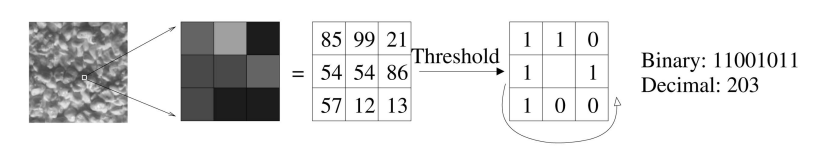
\includegraphics{obrazky-figures/lbp.png}}
  \label{lbp}
  \caption{Ukázka ohodnocení pixelu algoritmem LBP \cite{localBinaryPatterns}}
  \end{center}
\end{figure}

Algoritmus byl později vylepšen tak, aby uměl pracovat s~různě velkým okolím, které navíc nemusí mít čtvercový tvar. Používané okolí ve tvaru kružnice je popsáno dvojicí $(P, R)$, kde $P$ je počet vzorkovacích bodů a $R$ je poloměr kružnice. Další vylepšení LBP algoritmu se týkalo definování tzv. uniformních vzorů (anglicky uniform patterns). Tyto vzory jsou ty vzory v~nichž se vyskytují nejvýše 2 přechody z~1 na 0 a opačně. Příkladem uniformního vzoru na okolí $(8, 2)$ je 11100000 (1 přechod), či 00111000 (2 přechody). 

Lokální primitiva (obrázek \ref{lbpprimitives}) a histogramy vytvořené z~takto získaných hodnot se využívají mj. k~detekci obličejů.

\begin{figure}[H]
  \begin{center}
      \scalebox{0.8}{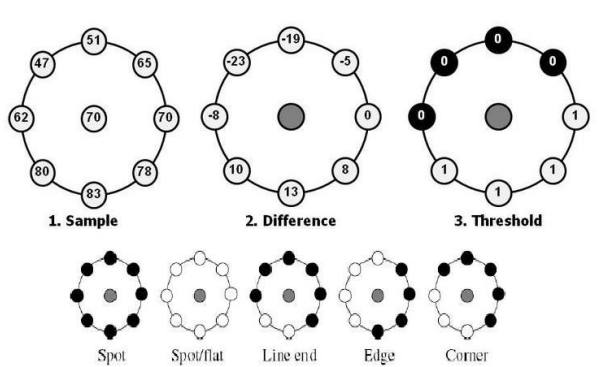
\includegraphics{obrazky-figures/lbpPrimitives.png}}
  \label{lbpprimitives}
  \caption{Lokální primitiva detekované algoritmem LBP \cite{localBinaryPatternsTests}}
  \end{center}
\end{figure}

\subsection*{Viola--Jones algoritmus}
\label{sekce:viola_jones}
Algoritmus \textbf{Viola--Jones} \cite{violaJonesArticle, violaJones}, někdy také nazývaný \textbf{Haar Cascades}, je obecně technika pro detekci objektů, vytvořená před používáním metod hlubokého učení. Používá se k~detekci obličejů, částí těla, očí, úst atd. Dosahuje přesnosti detekce kolem 90 \% \cite{violaJones}. 

Princip fungování algoritmu spočívá v~detekci hran a čár (obecně vlastností) v~černobílém obrázku (hodnoty pixelů jsou na intervalu $<0; 1>$). Vybere se jedna z~vlastností (některé z~nich zobrazuje obrázek \ref{haarfeatures}) a vypočítá se průměrná hodnota pixelů ve všech obdélnících (obdélníky jsou dva, tři nebo čtyři). Rozdíl těchto hodnot pak určuje zda se jedná o~hranu, čáru tzn. zda je daná vlastnost detekována. Pokud například budeme hledat vlastnost \emph{b)} z~obrázku \ref{haarfeatures} a vypočtený rozdíl hodnot je blízký 1, detekce byla úspěšná (viz ukázka v~obrázku \ref{haarexample}).

\begin{figure}[H]
  \begin{center}
      \scalebox{0.6}{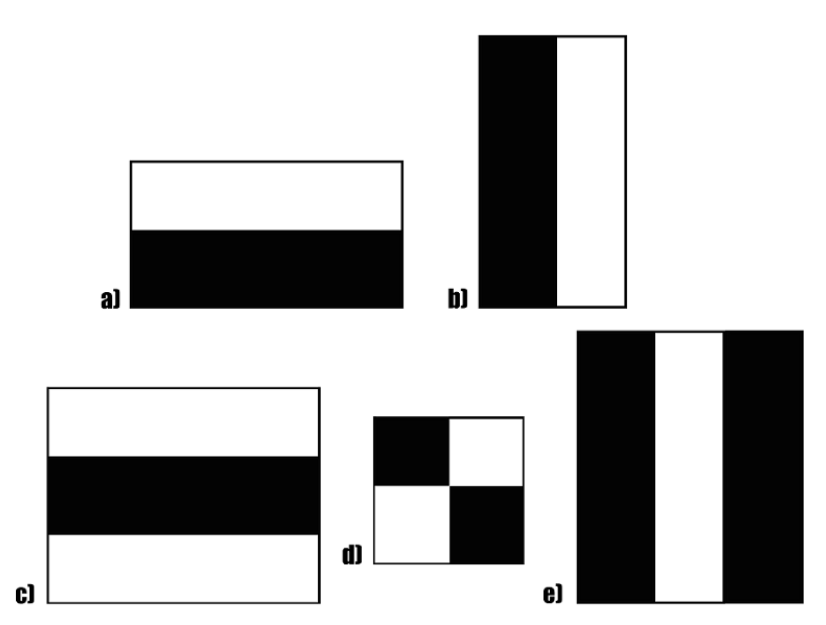
\includegraphics{obrazky-figures/haarfeatures.png}}
  \label{haarfeatures}
  \caption{Haarovy vlastnosti \cite{violaJonesArticle}
  a) horizontální hrana; b) horizontální hrana; c) horizontální čára d) diagonála e) vertikální čára}
  \end{center}
\end{figure}

\begin{figure}[H]
  \begin{center}
      \scalebox{0.4}{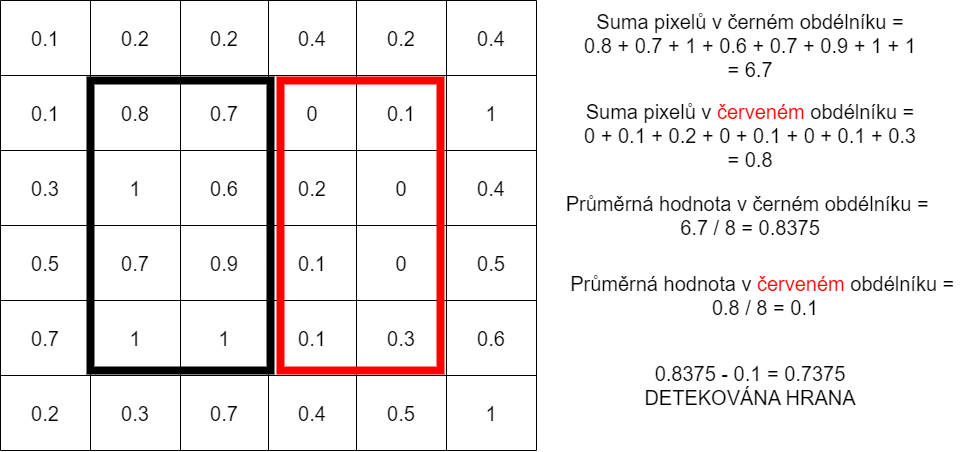
\includegraphics{obrazky-figures/haarexample.png}}
  \label{haarexample}
  \caption{Příklad výpočtu detekce hrany dle vlastnosti b) z~obrázku \ref{haarfeatures}. Bílý obdélník je nahrazen červeným pro lepší viditelnost.}
  \end{center}
\end{figure}

Algoritmus postupně prochází celý obrázek a hledá výskyt některé z~vlastností. Toto procházení u~obrázků s~velkým počtem pixelů znamená enormní výpočetní nároky, protože je potřeba vždy počítat s~hodnotami všech dotčených pixelů. Proto Viola a Jones \cite{violaJones} navrli
vylepšení nazvané anglicky \textbf{Integral Image}. To spočívá v~tom, že všechny pixely stačí projít pouze 1x, a každý tento pixel lze ohodnotit sumou hodnot pixelů směrem nalevo a nahoru (důsledkem je, že pixel s~nejnižším ohodnocení se nachází v~levém horním rohu a pixel s~nejvyšším ohodnocením v~pravém dolním rohu). Následný výpočet průměrné hodnoty ukazuje obrázek \ref{integralimage}. 

\begin{figure}[H]
  \begin{center}
      \scalebox{0.7}{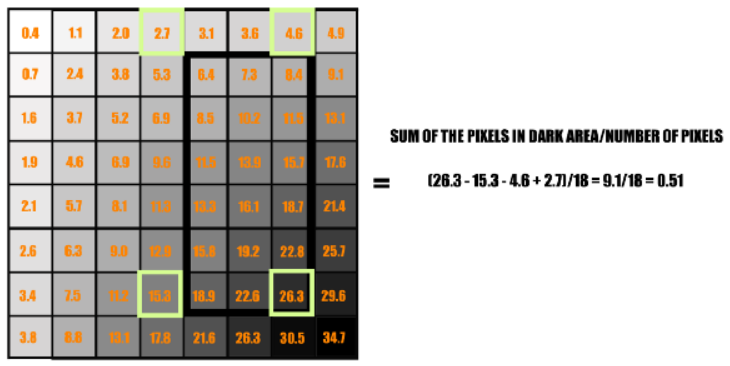
\includegraphics{obrazky-figures/integralimage.png}}
  \label{integralimage}
  \caption{Ukázka výpočtu hodnoty obdélníku v~Haarově vlastnosti za pomoci vylepšení \textbf{Integral Image} \cite{violaJonesArticle}.}
  \end{center}
\end{figure}

Jelikož Haarových vlastností je velké množství, bylo vybráno 6000 nejvíce vyhovujících, které se k~detekci obličejů používají. Detekce je rozdělena na několik etap, v~každé etapě je vyhledáván v~části obrázku výskyt několika vlastností (počet s~každou etapou roste), pokud se vyhledání nezdaří, není již dále daná část obrázku prohledávána. 


\subsection*{Histogram orientací gradientů}
Metoda HOG (anglicky Histograms of Oriented Gradients) \cite{hog, hog2} používá k~detekci obličejů či postav histogramy orientovaných přechodů v~obrázku, rozděleném dle mřížky na několik bloků (často například 8$\times$8 nebo 4$\times$4 pixelů). Pro každý pixel v~takovémto bloku jsou vypočítány hodnoty gradientů -- velikost (magnitude) a směr (direction). Tyto hodnoty jsou pak přiřazeny do jednoho či více sloupců v~histogramu popisujícím celý blok.

Tento histogram bývá rozdělen na 9 sloupců (rozmezí -- anglicky bin) vyjadřujících směr gradientu v~úhlu na škále od 0$^\circ$ do 180$^\circ$, kdy každý sloupec odpovídá intervalu 20$^\circ$. Výslednému vektoru, který udává velikosti gradientů v~jednotlivých úhlech se říká HOG deskriptor.

HOG využívá pro zlepšení detekce při zhoršených světelných podmínkách normalizaci HOG deskriptorů. Tato normalizace je prováděna na vektorech 4 sousedících bloků. Pokud je tedy vektor složen z~9 hodnot, vypočítá se normalizační vektor z~$9 \times 4 = 36$ hodnot.

Výsledkem metody je obrázek (viz obrázek \ref{hogexample} reprezentovaný orientovanými gradienty, který se využívá k~detekci osoby nebo obličeje.

\begin{figure}[H]
  \begin{center}
      \scalebox{0.5}{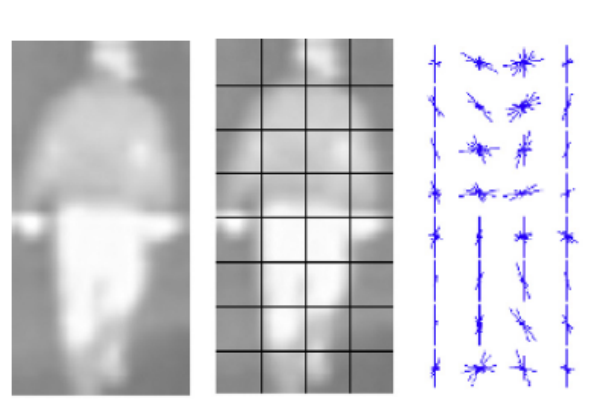
\includegraphics{obrazky-figures/hogexample.png}}
  \label{hogexample}
  \caption{Zleva výřez originálního obrázku převedený do šedotónové reprezentace, rozdělený obrázek na bloky, výstup metody HOG \cite{hog2}.}
  \end{center}
\end{figure}


%%%%%%%%%%%%%%%%%%%%%%%%%%%%%%%%%%%%%%%%%%%%%%%%%%%%%%%%%
%       KAPITOLA 3 - Neuronové sítě
%%%%%%%%%%%%%%%%%%%%%%%%%%%%%%%%%%%%%%%%%%%%%%%%%%%%%%%%%
\chapter{Neuronové sítě pro detekci obličeje}
\label{kapitola:neuronove_site}
Tato kapitola popisuje neuronové sítě a jejich využití pro detekci obličejů. Sekce \ref{sekce:NS} se věnuje popisu neuronových sítí obecně, v~sekci \ref{sekce:datasety} jsou popsány datasety a jejich využití k~trénování neuronových sítí. Sekce \ref{sekce:NSdetektory} se zabývá konkrétními detektory obličejů s~využitím neuronových sítí. Konkrétní programovací frameworky pro práci s~neuronovými sítěmi vyobrazuje sekce \ref{sekce:frameworky_pro_ns}.

\section{Neuronové sítě}
\label{sekce:NS}

Neuronové sítě \cite{deeplearningbook, ns1994} umožňují nalezení neznámého řešení problému pomocí naučení se z~podobných problémů u~nichž známe řešení. Tyto umělé sítě jsou inspirovány biologickou nervovou soustavou lidí (lidským mozkem). Síla neuronových sítí se projevuje v~úlohách zaměřených na detekci, rozpoznávání (objektů, lidí, obličejů, obecně vzorů -- anglicky patterns) a~zpracování dat. Existuje řada druhů neuronových sítí (konvoluční, hluboké, dopředné, rekurentní), pro detekci obličejů v~obrázcích se nejčastěji používají konvoluční neuronové sítě (anglicky Convolutional Neural Networks -- CNN). 

Na princip fungování neuronových sítí může být nahlíženo jako na nelineární matematickou funkci, která převádí $X$ vstupů na $Y$ výstupů. Proces transformace vstupních informací na výstup je ovlivňován váhováním hodnot vně sítě. Tyto hodnoty vah jsou určovány při tzv. učení/trénování neuronových sítí. Pro správné natrénování neuronové sítě je potřeba dostatečného počtu vstupních trénovacích dat (obrázků, textů, hodnot) a~dostatečně výkonný hardware. 

\subsection*{Biologický neuron}
Jak již bylo zmíněno, inspirací neuronových sítí je biologická nervová soustava. V~lidském mozku se nachází okolo $10^{11}$ neuronů (elektricky aktivních buněk spracovávajích signály). Vstupem těchto neuronů jsou tzv. dendrity, výstupy pak nazýváme axony. Jednotlivé neurony jsou navzájem propojeny tisíci spoji pojmenovanými synapse. Synapse zajišťují komunikaci mezi neurony.

Takto vytvořený paralelismus poskytuje mozku schopnost rychle zpracovávat informace. Neurony biologické i umělé pracují s~váhovanými vstupy. Po překročení určitého prahu na vstupech je adekvátně upraven výstup neuronu. Klíčovou vlastností potom je způsobilost měnit hodnoty jednotlivých vah na základě externích vlivů. Tím dochází k~učení sítě neuronů.

\subsection*{Perceptron}

Nejjednoduším modelem umělého neuronu je preceptron. Perceptron má $N$ vstupů, jejichž hodnoty $x$ jsou vynásobeny váhami $w$ a sesumovány dle vzorce \ref{vzorec:perceptron}.

\begin{equation} \label{vzorec:perceptron}
  a = \sum_{i=1}^{N} (w_i * x_i) + w_0 * x_0
\end{equation}

Hodnota $x_0$ se nazývá bias a jedná se o~neměnnou vstupní hodnotu (často má hodnotu $+1$). Váhy a vstupy (včetně biasu) mohou být jak kladné, tak i záporné. Hodnota $a$ je po vypočtení předána tzv. \textbf{aktivační funkci}.

\begin{figure}[H]
  \begin{center}
      \scalebox{0.4}{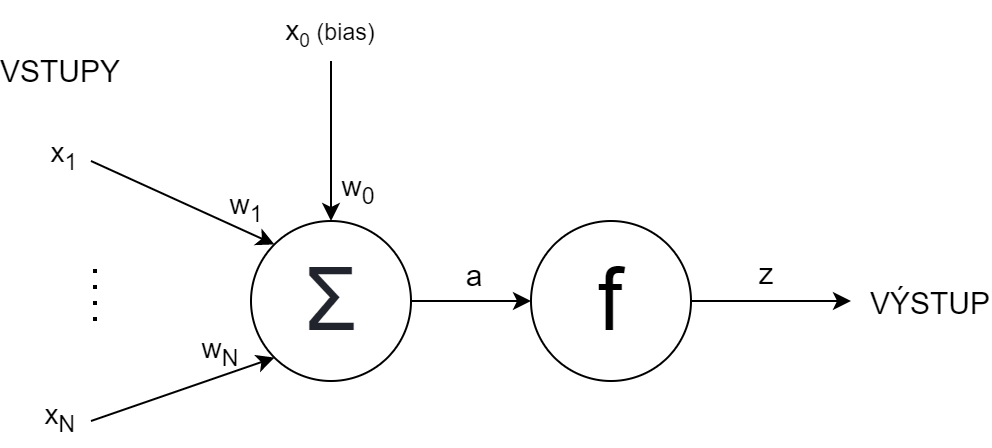
\includegraphics{obrazky-figures/perceptron.png}}
  \label{obrazek:perceptron}
  \caption{Perceptron s~N vstupy, biasem $x_0$ a aktivační funkcí $f$}
  \end{center}
\end{figure}

\subsection*{Aktivační funkce}
Aktivační funkce $f$ je matematická funkce, která určuje výstup neuronu (vzorec \ref{vzorec:aktivacni_fce}). Na výběru vhodné aktivační funkce závisí přesnost neuronové sítě. Funkce může být různá, pro příklad je zde uveden výstup rozlišující zda se jedná o~kladné či záporné číslo nebo nulu (viz vzorec \ref{vzorec:vystup_aktivacni_fce}). V~praxi se často používá aktivační funkce nazvaná \textbf{rectified linear unit} (ReLU) \cite{deeplearningbook} definovaná jako $f(a) = max\{0, a\}$.

\begin{equation} \label{vzorec:aktivacni_fce}
  z~= f(a)
\end{equation}

\begin{equation}
  \label{vzorec:vystup_aktivacni_fce}
   f(a) =
    \begin{cases}
      0       & \quad \text{pro } a = 0\\
      1       & \quad \text{pro } a > 0\\
      -1       & \quad \text{pro } a < 0
    \end{cases}
\end{equation}

\subsection*{Spojování neuronů}
Spojením několika neuronů lze vytvořit tzv. vrstvu (anglicky layer) perceptronů. Tytvo vrstvy se dělí na vstupní (anglicky input), výstupní (anglicky output) a skryté (anglicky hidden). Konkatenací vstupní, několika skrytých a výstupní vrstvy je možno vytvořit neuronovou síť připravenou k~trénování.

\begin{figure}[H]
  \begin{center}
      \scalebox{0.22}{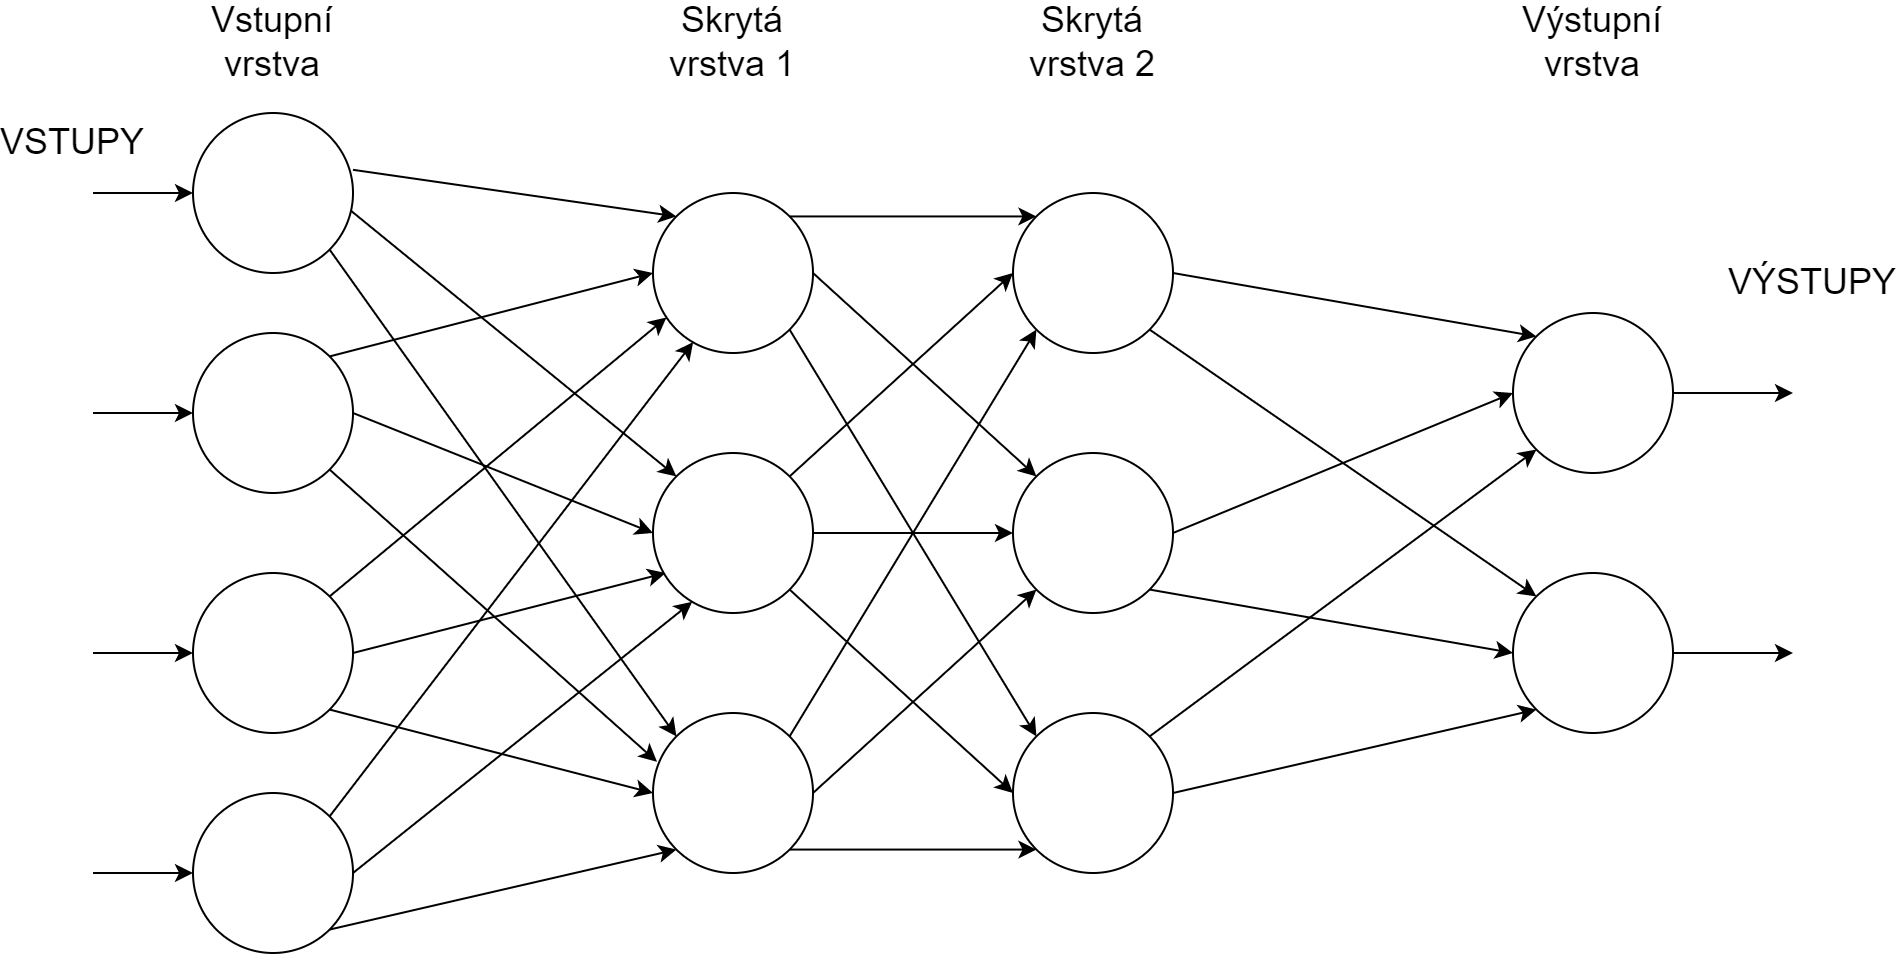
\includegraphics{obrazky-figures/nsexample.png}}
  \label{obrazek:nsexample}
  \caption{Propojení vrstev neuronů do neuronové sítě}
  \end{center}
\end{figure}

\subsection*{Učení}
Aby neuronová síť mohla fungovat, musí se natrénovat (tzn. nastavit co nejpřesněji váhy na vstupech neuronů). K~trénování se používají data z~datasetů (viz sekce \ref{sekce:datasety}). Trénování neuronových sítí lze rozdělit do 3 kategorií \cite{deeplearningbook}:

\begin{itemize}
  \item \textbf{Učení bez učitele} (anglicky unsupervised learning) -- tyto algoritmy procházejí data z~datasetu a provádějí nad nimi shlukování do tzv. clusterů.
  \item \textbf{Učení s~učitelem} (anglicky supervised learning) -- každým datům z~datasetu je přiřazena informace o~požadpvaném výstupu. Vstupy jsou zpracovány neuronovou sítí a podle chyby (rozdílu vstup/výstup) jsou upraveny parametry v~neuronové síti.
  \item \textbf{Posilované učení} (anglicky reinforcement learning) -- tento druh učení není vázán pouze na data z~datasetu, ale navíc interaguje s~prostředím.
\end{itemize}

Trénování neuronových sítí je rozděleno do tzv. \textbf{epoch}, kdy jedna epocha znamená, že všechna trénovací data byla zpracována neuronovou sítí právě jedenkrát. S pojemem epocha souvisí pojem \textbf{batch}, který udává počet trénovacích dat, které síť zpracuje, než dojde k aktualizaci jejích vnitřních stavů. Běžně používané hodnoty batch jsou mocniny 2 (2, 4, 8, 16, 32, 64). 

\subsection*{Chyby}
Abychom byli schopní aktualizovat váhy vstupů jednotlivých neuronů, je potřeba měřit chybovost výstupu neuronové sítě. Jednou z~možností měření chyby (využitelné například při lineární regresi) je \emph{mean squared error}. Dle vztahu \ref{vzorec:mse} je vypočítána chybovost a jsou upraveny váhy. Snahou je chybu co nejvíce zmenšit.

\begin{equation}
  \label{vzorec:mse}
  MSE = \frac{1}{N} \sum_{i}^{N} (vystupNS - spravnyVystup)^2
\end{equation}

Při trénování může dojít k~situaci, kdy neuronová síť zvládá zpracovávat trénovací data s~velmi vysokou přesností, ale při použití testovacích (validačních) dat se chybovost zvyšuje. V~takovémto případě mluvíme o~\textbf{přetrénování} (anglicky overfitting). Druhým nežádoucím jevem, který může nastat je \textbf{nedotrénovanost} (anglicky underfitting) -- síť není dostatečně natrénovaná a dochází tak k~vysoké chybovosti (příčinou je například málo trénovacích dat).


\begin{figure}[H]
  \begin{center}
      \scalebox{0.18}{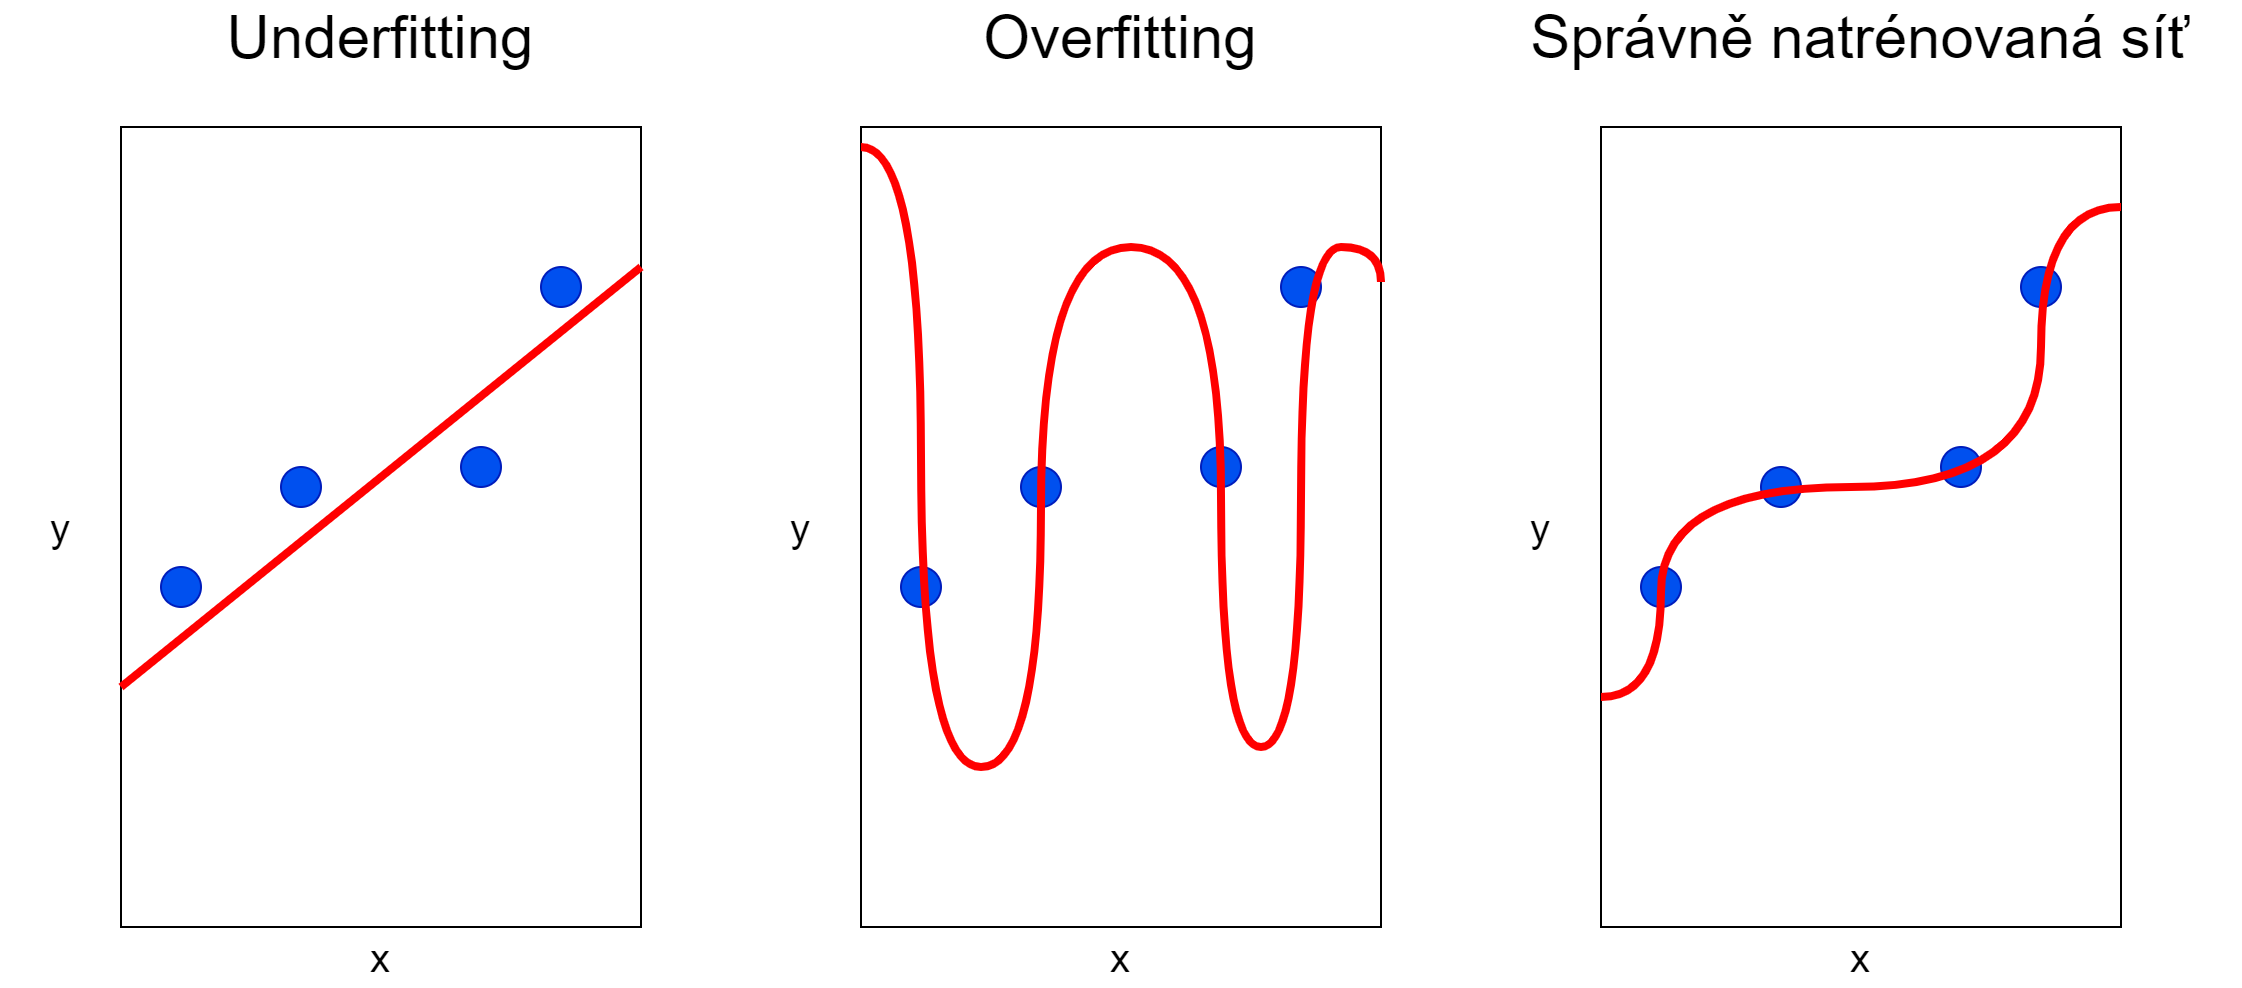
\includegraphics{obrazky-figures/fitting.png}}
  \label{obrazek:fitting}
  \caption{Ukázka výstupu neuronové sítě při nedoučení, přeučení a dostatečně dobrém množství dat pro učení}
  \end{center}
\end{figure}


\section{Datasety}
\label{sekce:datasety}
Datasetem rozumíme soubor podobných dat (například obrázků obličejů, číslic, předmětů nebo textů). Pro detekci obličejů se využívají datasety obsahující fotografie a videa lidí z~veřejně dostupných zdrojů (internet, televize) nebo jsou datasety přímo účelně vytvářeny (fotografování lidí) a následně je možné si je koupit nebo stáhnout. Data v~datasetech je nutné tzv. anotovat (označit co na daném obrázku je). V~případě tváří se může jednat například o~věk osoby, pohlaví, rasu, aby bylo možné určit zda po klasifikaci neuronovou sítí výstup odpovídá požadovanému výsledku. Následující podsekce popisují datasety používané k~učení neuronových sítí pro detekci obličejů.

\subsection*{Datasety lidských obličejů}
Dataset \textbf{WIDER FACE}\footnote{\url{http://shuoyang1213.me/WIDERFACE/}} je dataset snímků obličejů obsahující 32203 obrázků ve skupinách trénovací, validační, testovací s poměrovým rozdělením 40\%/10\%/50\%. Dataset je volně přístupný a autoři poskytují k trénovacím a validačním obrázkům anotační soubory s pozicemi obličejů. Fotografie spadají do různých skupin jako jsou různé pozice hlavy, různé zakrytí obličeje nebo špatné světelné podmínky. Fotografie jsou navíc rozděleny do 61 kategorií podle událostí, za kterých byly pořízeny (například demonstrace nebo volby).

\begin{figure}[H]
  \begin{center}
      \scalebox{0.6}{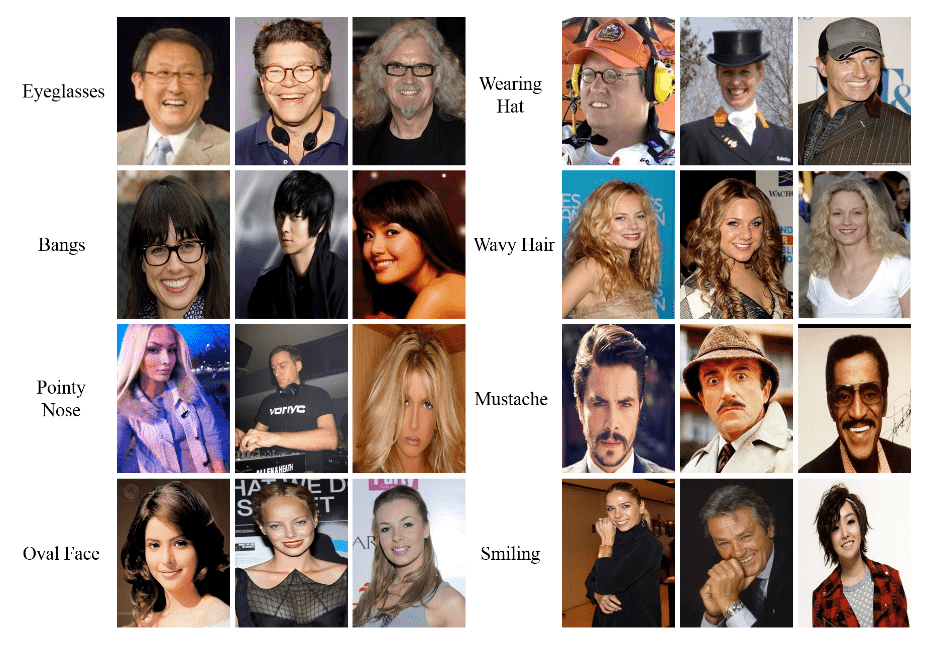
\includegraphics{obrazky-figures/celeba.png}}
  \label{obrazek:celeba}
  \caption{Příklady obličejů z~datasetu WIDER FACE}
  \end{center}
\end{figure}

Dataset \textbf{DigiFace1M} \cite{digiface1m} se skládá z~1 milionu snímků digitálně vytvořených obličejů (viz obrázek \ref{obrazek:digiface}), čímž se vyhýbá případným právním a etnickým problémům, které mohou být spojeny s~využití tváří reálných osob. Při použití tohoto datasetu umělých tváří společně s~200 až 2000 fotografiemi tváří reálných lidí pro učení, lze dosáhnout podobných výsledků detekce jako s~datasety tvořenými čistě reálnými obličeji.

\begin{figure}[H]
  \begin{center}
      \scalebox{0.6}{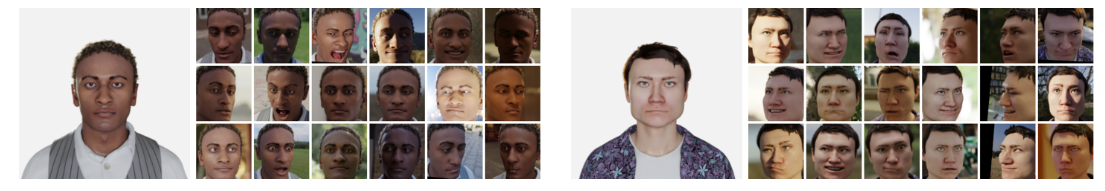
\includegraphics{obrazky-figures/digiface.png}}
  \label{obrazek:digiface}
  \caption{Příklady vygenerovaných obličejů pod různými úhly a různým osvětlením z~datasetu DigiFace1M \cite{digiface1m}}
  \end{center}
\end{figure}

\textbf{Multi-PIE} \cite{multipie} je dataset zaměřený na fotografie obličejů pořízených za různých světelných podmínek a pod různými úhly. Obshauje přes 750000 snímků, které byly vytvořeny vyfotografováním 337 lidí po dobu několika měsíců. Tento dataset je placený.

Dataset \textbf{UTKFace} \cite{utkface} obsahuje přes 20000 fotek obličejů lidí různých věků, pohlaví a~ras z~různých úhlů a~za rozličných světelných podmínek. Dataset je volně dostupný pro nekomerční použití. Data jsou podrobně anotovány dle vzorce \texttt{[věk]\_[pohlaví]\_[rasa]\_
[datum a čas].jpg}, kde věk je v~rozmezí 0--116 let, pohlaví muž/žena, rasa je jedna z~výčtu běloch, černoch, asiat, ind, ostatní a datum a čas uchovává informaci o~okamžiku zařazení fotografie do datasetu.

Dataset \textbf{DARK FACE} \cite{darkFace} obsahuje 6000 fotografií různých prostředí s~lidmi, pořízených za špatných světelných podmínek. Používá se mj.při hodnocení účinnosti detektorů obličejů. Dataset obsahuje jak anotované tak neanotované obrázky.

\section{Detektory obličeje}
\label{sekce:NSdetektory}

Jak již bylo zmíněno, detekce obličeje je jak samostatnou disciplínou, tak i vstupním bodem několika dalších analyzačních úkonů (rozpoznávání tváře, ověřování pomocí obličejů nebo identifikace obličejů). Zpracovávaný obrázek bývá rozdělen na několik menších oblastí (výřezů) a tyto výřezy bývají zpracovávány jednotlivě. 
Existuje řada různých druhů a architektur neuronových sítí využívaných k~detekci obličejů \cite{fdReviewNS}. Patří mezi ně například:

\begin{itemize}
  \item \textbf{Rotation invariant neural network} (RINN, rotačně invariantní neuronová síť) -- dokáže detekovat obličeje bez ohledu na úhel natočení tváře (není nutná normalizace v~preprocessingu). Systém tohoto typu neuronové sítě obsahuje několik sítí, s~tím že první se nazývá \emph{router network}. Tato síť určuje orientaci (natočení) výřezu obrázku a~připravuje (normalizuje) tak výřez pro 1 či více detekčních sítí.
  \item \textbf{Fast neural network} (FNN, rychlá neuronová síť) -- obrázek je rozdělen na malé podobrázky a každý podobrázek je zvlášť otestován na výskyt tváře rychlou neuronovou sítí. Cílem je snížení výpočetního času nutného pro nalezení obličeje.
  \item \textbf{Polynomial neural network} (PNN, polynomiální neuronová síť) -- oblasti v~obrázku jsou klasifikovány jako tvář/ne--tvář pomocí binomické projekce této oblasti do podprostoru vlastností obličeje naučeného tzv. základní analýzou komponent (anglicky principal component analysis, PCA). Zkoumáním vlivu PCA na vzorky lze detekovat zda se jedná o~obličej.
  \item \textbf{Convolutional neural network} (CNN, konvoluční neuronové sítě) -- samostatně popsány v~další podsekci. 
\end{itemize}


\subsection*{Konvoluční neuronové sítě}
Konvoluční neuronové sítě (CNN) \cite{cnnNlp, cnnCv, cnnIntro} jsou použity ve většině systémů v~oblasti počítačového vidění. Jelikož můžeme hodnoty pixelů vyjádřit čísly (používá se šedotónová varianta obrázku $\rightarrow$ při 8 bitové barevné hloubce může pixel nabývat hodnot 0 -- 255), lze tyto čísla použít jako vstupy neuronové sítě. Při vysokém rozlišení obrázku však nastává problém. Pokud bychom chtěli každou hodnotu pixelu použít na vstupu neuronové sítě pro celý obrázek naráz, měla by neuronová síť již u~obrázku s~rozměry 500 $\times$ 500 pixelů celkem 25000 vstupní neuronů, což je příliš výpočetně náročné. Proto se využívá konvoluce.

\textbf{Konvoluce} je okenní matematická funkce, při níž je na každou část obrázku (okno, \emph{window}) násobením aplikována matice (filtr, kernel, konvoluční jádro). Princip konvoluce zachycuje následující obrázek.

\begin{figure}[H]
  \begin{center}
      \scalebox{0.25}{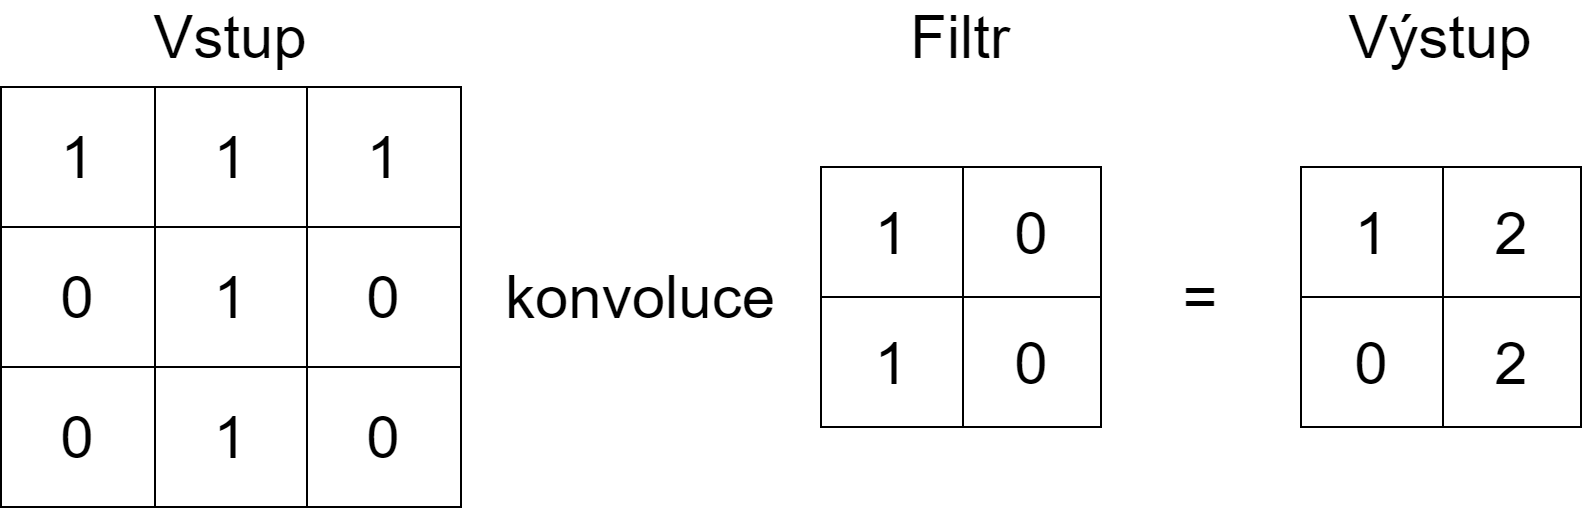
\includegraphics{obrazky-figures/principkonvoluce.png}}
  \label{obrazek:principkonvoluce}
  \caption{Princip konvoluce 2D obrázku s~rozměry 3$\times$3 a filtru $2\times2$}
  \end{center}
\end{figure}

Konvoluce dovoluje zásadně snížit počet nutných vstupů neuronové sítě. Navíc jsou konvoluční operace rychlé, protože tato funkce je hardwarově implementována na grafické kartě.

Jak lze vidět na obrázku \ref{obrazek:cnnpipeline} konvoluční neuronová síť se skládá z~několika vrstev.

\begin{figure}[H]
  \begin{center}
      \scalebox{0.55}{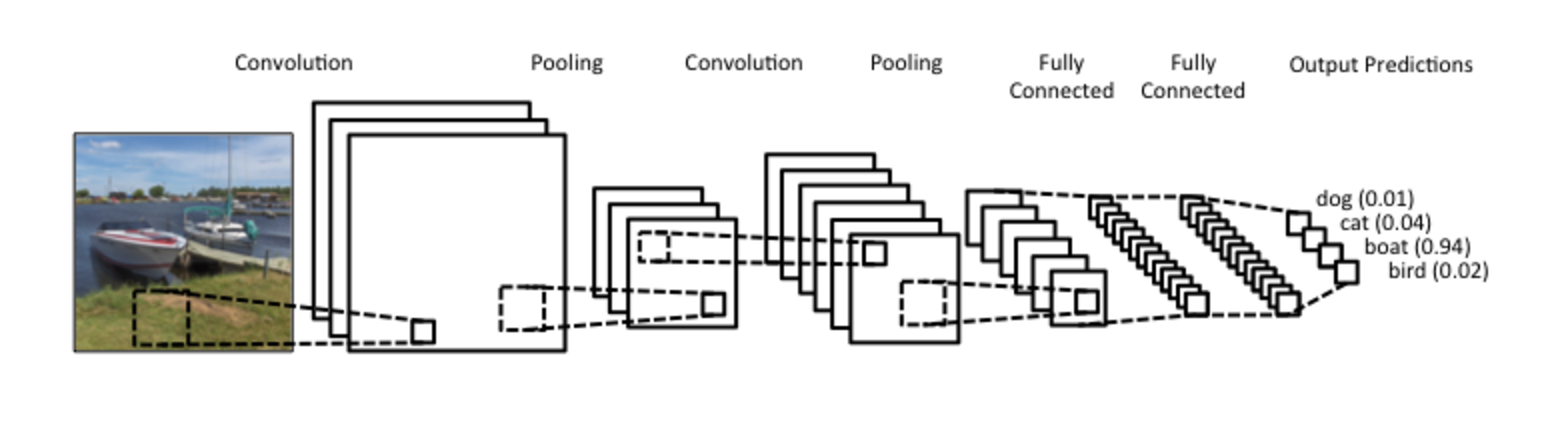
\includegraphics{obrazky-figures/cnnpipeline.png}}
  \label{obrazek:cnnpipeline}
  \caption{Řetězec vrstev konvoluční neuronové sítě \cite{cnnNlp}}
  \end{center}
\end{figure}

\textbf{Konvoluční vrstva} provádí výše popsanou konvoluci. Otázkou zůstává jak zpracovávat okraje obrázku. Existují dva přístupy:

\begin{itemize}
  \item \emph{Wide convolution} -- přidání nul kolem dokola obrázku a provedení konvoluce krajních hodnot (výstup bude stejně velký jako vstup).
  \item \emph{Narrow convolution} -- provedení konvoluce jako na obrázku \ref{obrazek:principkonvoluce}. Dojde ke zmenšení velikosti na výstupu.
\end{itemize}

Dalším parametrem konvolučních neuronových sítí je tzv. \textbf{stride} velikost. Určuje o~kolik hodnot se konvoluční jádro posune při každém kroku. Na obrázku \ref{obrazek:principkonvoluce} je použit stride 1. Větší hodnota stride vede k~menšímu výstupu. Běžně se používají hodnoty 1 nebo 2.

\textbf{Poolingová vrstva} (anglicky pooling layer) je vrstva aplikovaná po konvoluční vrstvě. Používá se ke snížení výpočetní náročnosti. Tím, že je aplikována statistická funkce (maximum, průměr) na výstup konvoluční vrstvy (většinou filtrem o~velikosti 2 $\times$ 2 se stride = 2), dojde ke zredukování počtu hodnot výsledné matice (viz obrázek \ref{obrazek:cnnpooling}).

\begin{figure}[H]
  \begin{center}
      \scalebox{0.25}{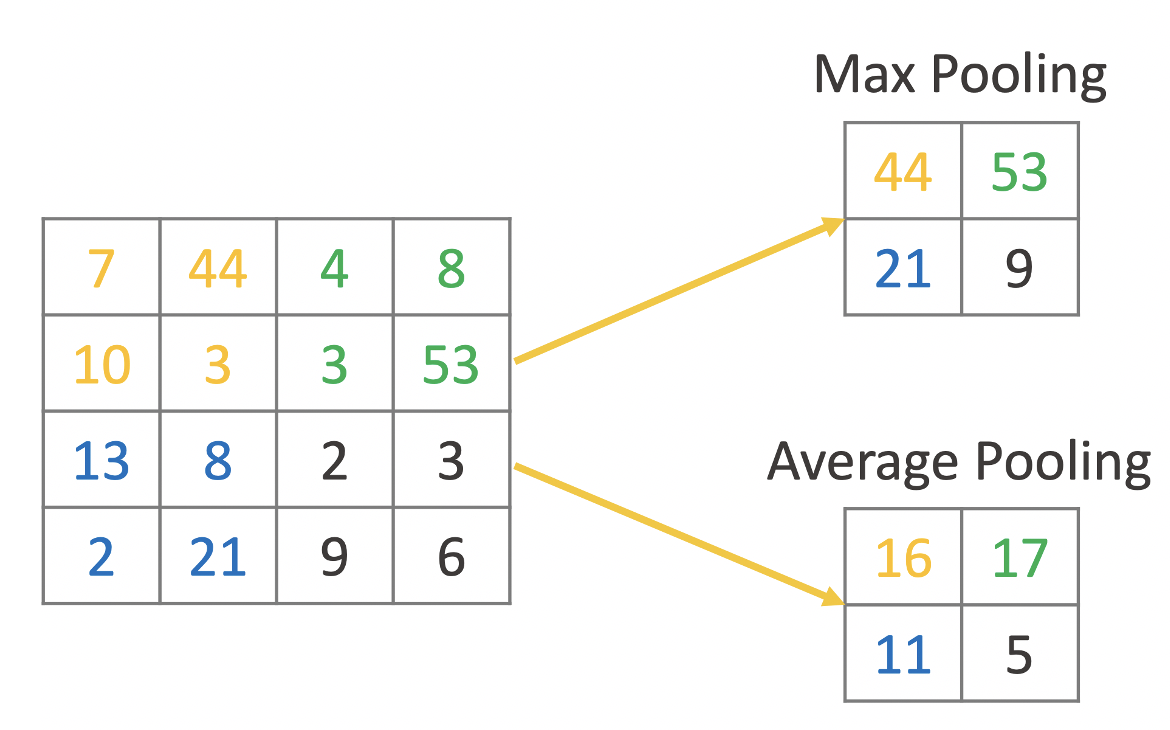
\includegraphics{obrazky-figures/cnnpooling.png}}
  \label{obrazek:cnnpooling}
  \caption{Řetězec vrstev konvoluční neuronové sítě \cite{cnnCv}}
  \end{center}
\end{figure}

V~reálné aplikaci jsou konvoluční a poolingové vrstvy poskládány za sebe. Na konci řetězce (obrázek \ref{obrazek:cnnpipeline}) se pak nachází část plně propojených vrstev neuronů (fully--conected layer).

\subsection*{Detektory}
Tato část popisuje vybrané existující detektory obličejů založené na neuronových sítí a~porovnání úspěšnosti detekce těchto detektorů s~detektory popsanými v~sekci \ref{sekce:detektory_bez_neuronovych_siti}.

\textbf{MTCNN} (Multi-Task Cascaded Convolutional Network) \cite{fdCNNComparison, MTCNN} provádí detekci obličejů pomocí kaskády konvoluční neuronových sítí. Algoritmus má dvě části. První část vytváří několik verzí vstupních obrázků, každa taková verze má jiné rozlišení. Druhá část složená z~kaskády neuronových sítí se stará o~detekci obličeje v~různých verzích obrázku. Použití více verzí obrázku umožňuje zvýšit efektivitu detekce.

Single shot detector \textbf{SSD} \cite{ssd} je konvoluční neuronová síť opět složená ze 2 částí, sloužící obecně k~detekci objektů. Tyto části jsou: a) natrénovaný detekční model (VGG--16 nebo jiný) a b) část SSD -- další konvoluční vrstva, která rozděluje obrázek pomocí mřížky (\emph{grid}) s~rozměry 4 $\times$ 4 nebo 8 $\times$ 8. V~každém takto vytvořeném bloku je pak hledán objekt (obličej).

Detekční model \textbf{RetinaFace} \cite{lowLightFdReview} používá multitasking pro učení. Detekce probíhá určením pozice obličeje podle vyhledání pixelů, které tvář obsahuje. Model má 2 struktury: \emph{Multi--task loss} -- minimalizace chyb modelu a \emph{Dense Regression Branch} -- renderer, který filtruje obličeje a získává pixely z~vyrenderovaných obličejů.

\textbf{YOLO} (You Only Look Once) \cite{yolo} je stejně jako SSD tzv. single shot detektor -- rozděluje vstupní obrázek do mřížky a provádí detekci případně rekognici nad jednotlivými bloky mřížky. Pro každý blok je určena hodnota jistoty výskytu objektu. Na vstupu sítě YOLO jsou barevné obrázky o~velikosti 448 $\times$ 448 pixelů. Architektura neuronové sítě je složena ze 7 konvolučních vrstev následovaných pooling vrstvami a 3 plně propojenými vrstvami na výstupu.
YOLO má několik verzí, které se liší složením neuronové sítě a úspěšností detekce.

\subsection*{Porovnání výkonnosti detektorů}
Práce \cite{fdCNNComparison} se zabývá porovnáním detektorů Viola--Jones, Histogram of Oriented Gradients ze sekce \ref{sekce:detektory_bez_neuronovych_siti} a algoritmů založených na konvolučních neuronových sítích MTCNN a SSD (detektor VGG--16 je nahrazen detektorem MobileNet) ze sekce \ref{sekce:NSdetektory}. Testování bylo prováděno na datasetech AFW a WIDER FACE. Co se týká úspěšnosti detekce, nejlépe vyšel z~testu detektor MTCNN, nejrychlejší pak byl detektor SSD (viz obrázek \ref{obrazek:cnncomparison}). Z~detektorů založených na klasických metodách měl vyšší úspěšnost HOG, rychlejší však byl detektor Viola--Jones. Hodnota AP (average precision) udává průměrnou přesnost detekce a hodnota FPS (frames per second) počet snímků zpracovaných za sekundu.

\begin{figure}[H]
  \begin{center}
      \scalebox{0.7}{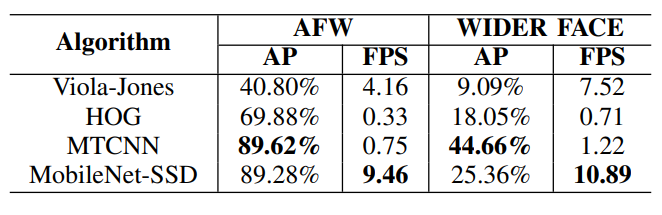
\includegraphics{obrazky-figures/cnncomparison.png}}
  \label{obrazek:cnncomparison}
  \caption{Výsledek testování detekčních algotitmů \cite{fdCNNComparison}.}
  \end{center}
\end{figure}

\subsection*{Detektory zaměřující se na špatné světelené podmínky}
Detektory zaměřující se na detekci ve špatných světelných podmínkách jsou buď specializované detektory, kdy je neuronová síť detektoru učena na datasetu vhodných obrázků (obrázky pořízené za špatných světelných podmínek) nebo je použit detektor obličeje natrénovaný na obyčejných snímcích. V~obou případech je nutno nejprve provést \emph{low--light image enhacement} (vylepšení obrázku) a~až poté přejít k~detekci.

Pro vylepšení obrázku existují různé metody \cite{lowLightFdReview}:
\begin{itemize}
  \item Mirnet,
  \item Adaptive Gamma Correction (AGC),
  \item Retinex,
  \item RetinexNet,
  \item a další.
\end{itemize}

\textbf{Mirnet} je metoda postavená na konvolučních neuronových sítí a jejím cílem je zvýšení kvality obrazu pomocí několika úprav v~konvolučních vrstvách.

\textbf{AGC} je metodou využívající gamma korekci k~vylepšení nasvícení scény (obrázku). Metoda navíc rozděluje obrázky podle intenzity gamma na tmavé (hodnota pod $0,5$) a~světlé (hodnota nad $0,5$).

Koncept \textbf{Retinex} se snaží upravit kvalitu obrazu tak, aby odpovídala kvalitě lidského vidění. Dosaženo toho je tak, že je prováděno odmazávání odrazů světla z~obrázku.

\textbf{RetinexNet} vychází z~Retinexu a provádí dekompozici obrázku tak, aby došlo k~oddělení odrazů nezávislých na osvětlení a osvětlení se známou strukturou. Metoda také celkově upravuje nasvícení pro dosažení co největší konzistence světla v~obrázku.

Pro porovnání účinnosti \emph{image enhacement} metod lze použít 2 veličiny. \emph{Peak signal--noise ratio} (PSNR)-- poměr užitečného signálu k~šumu a~\emph{Structural similarity} (SSIM) -- index podobnosti 2 obrazů.

\begin{figure}[H]
  \begin{center}
      \scalebox{0.45}{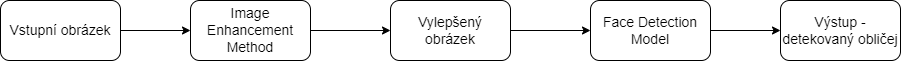
\includegraphics{obrazky-figures/iepostup.png}}
  \label{obrazek:iepostup}
  \caption{Řetězec postupu detekce obličeje ve zhoršených světelných podmínkách. Vychází z~\cite{lowLightFdReview}.}
  \end{center}
\end{figure}

Obrázek \ref{obrazek:iepostup}, který vychází ze článku \cite{lowLightFdReview} popisuje potřebný postup pro úpravu obrázku (preprocessing) a následné kroky vedoucí k~detekci obličeje. V~rámci tohoto článku jsou zpracovány výsledky detekce pomocí výše zmíněných metod vylepšení obrazu a detektoru RetinaFace (viz sekce Detektory). Jako testovací dataset byl použit dataset DARK FACE, popsaný v~sekci \ref{sekce:datasety}. V~rámci testování preprocessingových metod vylepšení obrazu bylo zjištěno, že nejlepší hodnoty PSNR ($19,48\:dB$) a SSIM ($0,74$) dosahuje metoda Mirnet (hodnoty dalších metod viz obrázek \ref{obrazek:psnrssim}).

\begin{figure}[H]
  \begin{center}
      \scalebox{0.7}{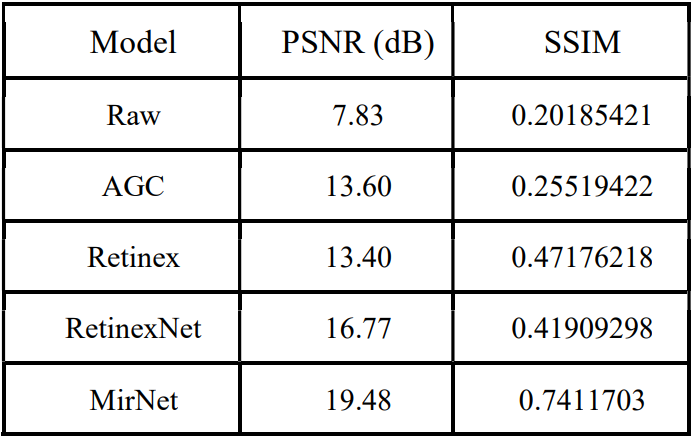
\includegraphics{obrazky-figures/psnrssim.png}}
  \label{obrazek:psnrssim}
  \caption{Hodnoty PSNR a SSIM pro metody vylepšení obrazu \cite{lowLightFdReview}.}
  \end{center}
\end{figure}

Výsledky detekce však ukázaly, že v~detekci obličejů si nejlépe vedl Retinex s~$0,43\:\%\:mAP$ (mean average precision -- průměrná přesnost detekce). Z~toho vyplývá, že lepší preprocessingová metoda nutně neznamená úspěšnější detektor.

Detekcí ve špatných světelných podmínkách se zabývá také článek \cite{HLAFace}. V~rámci tohoto článku byl vytvořen samoučící se (self--supervised) detektor dosahující $44,4\:\%\:mAP$ také na datech z~datasetu DARK FACE.

Práce \cite{fdExtremelyLowConditions} se rovněž zabývá detekcí nad datasetem DARK FACE při špatném osvětlení. Navržený algoritmus dosahuje $82,3\:\%\:mAP$. Algoritmus využívá 3 hlavní části umožňující dosáhnutí takto vysoké přesnosti detekce. Jsou to: \emph{Multi--scale retinex with color restoration} -- metoda podobná Retinexu, ale zachovává konzistenci barev, architektura konvolučních vrstev \emph{PyramidBox} a~\emph{Multi--scale test module} -- úpravy velikosti vstupního obrázku pro lepší detekci.

Velké rozdíly v~hodnotách $mAP$ jsou způsobeny tím, že neuronové sítě z~prací \cite{HLAFace, fdExtremelyLowConditions} jsou trénovány přímo na datasetu obličejů ve zhoršených pozorovacích podmínkách (specializoavné detektory), zatímco \cite{lowLightFdReview} používá model učený na běžných snímcích tváří.

\section{Frameworky pro neuronové sítě}
\label{sekce:frameworky_pro_ns}
Při programování neuronových sítí nebo obecně aplikací strojového učení se využívají k~tomu určené frameworky. Každý framework je trochu jiný a používá se k~jiným účelům. Všechny zde zmíněné frameworky podporují programovací jazyk Python. Mezi nejpoužívanější frameworky patří: TensorFlow, PyTorch, Keras, ONNX, Caffe \cite{nsFrameworks}.

\vspace{1em}
\textbf{TensorFlow} je framework pro jazyky R, C++, Python a další. Má několik modulů s~rozličnými funkcionalitami. Je velmi rozšířený a implementuje jej například Google překladač. Dokumentace je velmi podrobná a framework podporuje paralelismus napříč GPU.

\textbf{PyTorch} je vědecký framework použitelný v~jazyce Python, vhodný na prototypování. Navíc podporuje GPU paralelismus.

Dalším frameworkem je \textbf{Keras}, v~němž se programují konvoluční a rekurentní neuronové sítě. Je minimalistický a snadno se integruje spolu s~TensorFlow.

Framework \textbf{ONNX} je open source framework pro hluboké učení. Modely vytvořené v~ONNX lze konvertovat do jiných frameworků (TensorFlow, Keras).

\textbf{Caffe} je framework podporovaný napříč různými programovacími jazyky (C, C++, Python, MATLAB) a je vhodný pro konvoluční neuronové sítě. Umožňuje nastavit parametry sítě a natrénovat síť, není nutné ji přímo vytvářet.

V~rámci této práce jsou použity frameworky TensorFlow a Keras. 


%%%%%%%%%%%%%%%%%%%%%%%%%%%%%%%%%%%%%%%%%%%%%%%%%%%%%%%%%
%       KAPITOLA 4 - Systémy pro detekci a akcelerace detekce
%%%%%%%%%%%%%%%%%%%%%%%%%%%%%%%%%%%%%%%%%%%%%%%%%%%%%%%%%
\chapter{Systémy pro detekci obličejů a~akcelerace detekce}
\label{kapitola:kamery_a_systemy}
Detekci obličejů s~využitím počítačových programů lze provádět nad snímkem 
(fotografií, obrázkem), sadou snímků,
videozáznamem nebo tzv. real\,--\,timově pomocí kamer a kamerových systémů.
V~této kapitole jsou popsány aktuálně využívané prostředky pro vytváření 
obrázků k~detekci obličejů (kamery) a také dostupná řešení zabývající se 
detekcí, a to jak placené komerční, tak neplacené open--source systémy.

\section{Kamery}
Nezbytnou součástí oboru detekce obličejů jsou kamery a kamerové systémy.
Existují kamery specializované k~detekci či rozpoznávání obličejů 
a kamery obyčejné, které pouze zprostředkovávají obraz dále ke zpracování.

Specializované kamery se používají například k~zabezpečení objektů nebo
jako domovní videozvonky, kdy kamera (respektive její software) v~zachyceném
obraze detekuje a rozpozná obličej, a následně může vykonat přiřazenou akci 
(spustit alarm, poslat notifikaci, umožnit osobě vstup...) \cite{securityCamsWeb}.

Další oblastí, kde se kamery s~detekcí a rozpoznáváním obličejů uplatní je
bezesporu dohled ve veřejných prostorech (anglicky CCTV surveillance). 
Detekce obličeje může sloužit k~hledání podezřelých osob v~záznamech z~dohledových
kamer. Tyto záznamy jsou shromážďovány na serveru, pomocí detekce jsou
z~obrazu vyřezány fragmenty s~obličeji lidí a poté jsou tyto fragmenty
porovnány rozpoznávacím algoritmem s~obličeji hledaných osob. Při shodě
dochází k~informování administrátora systému, který podnikne další kroky 
\cite{suspectIdentification}. 

Kamery tedy mají v~doméně detekce obličejů nezastupitelnou roli, na 
jejich praktické využití v~systémech a řešení pro detekci se zaměřuje následujících
podkapitola.

\section{Dostupná řešení}
Řešení umožňující detekci (a často i rekognici) obličejů lze rozdělit do dvou kategorií: 
komerční (placené, profesionální) a nekomerční (zdarma, open--source, amatérské).
V~následujících dvou podsekcích jsou popsány konkrétní systémy umožňující
detekci obličejů včetně jejich výhod a nevýhod.

\subsection*{Komerční}
Komerčně využívaná zařízení pro detekci, případně rekognici lze běžně zakoupit 
a používat ve firemním nebo domácím prostředí. Mezi zástupce těchto zařízení
patří například produkty firem Netatmo, Google, Nest \cite{securityCamsWeb2}.

\begin{figure}[H]
  \begin{center}
      \scalebox{0.5}{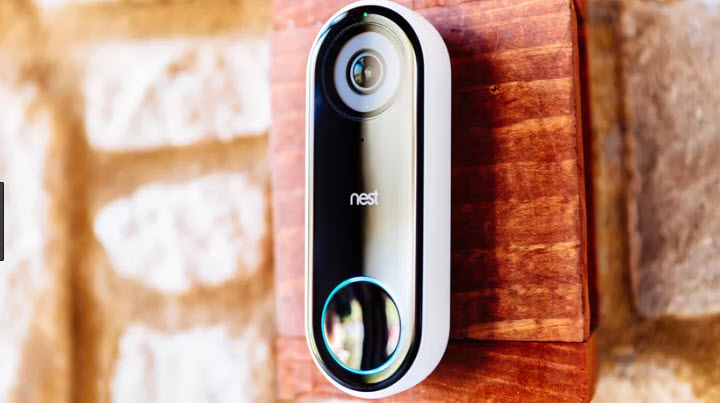
\includegraphics{obrazky-figures/nest-hello.png}}
  \label{nest}
  \caption{Nest Hello \cite{securityCamsWeb2}}
  \end{center}
\end{figure}

\subsection*{Nekomerční}
Nekomerční řešení pro detekci obličejů zahrnují frameworky s~otevřeným zdrojovým
kódem (open--source). Tyto frameworky a řešení využívají neuronové sítě, které jsou trénovány
pomocí datasetů a následně jsou využity k~detekci obličeje 
\cite{faceRecognitionFrameworks}.
Mezi open--source řešení patří například TinaFace \cite{TinaFace} nebo MTCNN \cite{MTCNN}, další volně použitelné frameworky popisuje sekce \ref{sekce:frameworky_pro_ns}.


\section{Akcelerace detekčních algoritmů}
\label{sekce:akcelerace}

S~rozmachem využívání strojového učení a neuronových sítí se objevila potřeba zrychlení těchto sítí. Proto byly vytvořeny specializované zařízení s~cílem urychlit výpočty a snížit energetickou náročnost výpočtů ve srovnání s~běžnými (univerzálními) výpočetním prostředky. Vznikly tak hardwarové akcelerátory neuronových sítí. Příkladem jsou Intel Neural Compute Stick 2 \cite{ncs2}, Coral \cite{coral} nebo Nvidia Jetson \cite{jetson}.

Existují různé typy architektur akcelerátorů \cite{acceleratorsSurvey}, mezi něž patří architektury popsané v~tomto odstavci.
\textbf{NPU} (neural processing unit) -- k~provádění matematických operací využívají speciální NPU obsahující PE (processing engines). NPU používá hardwarové verze MLP (multi--layer perceptron), pro dosažení zrychlení obecného výpočtu (nejen neuronových sítí). Pokud je část programu určená ke zrychlení spouštěna často a jsou dobře známy vstupy a výstupy, lze tuto část programu zrychlit pomocí NPU. Příkladem algoritmu pro zrychlení je rychlá Fourierova transformace (FFT).

Architektura \textbf{RENO} využívá memristory (ReRAM) -- speciální druh paměti jejíž struktura umožňuje urychlit maticové a vektorové násobení.

Mezi další akcelerátory patří série akcelerátorů \textbf{DianNao} využívaná na akademické půdě. Tyto akcelerátory obsahují NFU (neural functional unit), vstupní, výstupní a synaptický buffer a kontrolní procesor.

Průmyslovým akcelerátorem od Google je \textbf{TPU} (tensor processing unit). Je použitelný i přes cloud.

Kromě ReRAM jsou v~akcelerátor používány i paměti typu HMC (hybrid memory cube). Obě paměti (ReRAM a HMC) umožňují tzv. \emph{processing--in--memory}, takže snižují čas výpočtu tím, že není nutno data přesouvat mezi procesorem a pamětí. Příklady akcelerátorů postavených na HMC je Neurocube \cite{neurocube} nebo Tetris \cite{tetris}.

Většina akcelerátorů je zaměřena na výpočty s~již natrénovanou neuronovou sítí, jen pár jich podporuje učení neuronových sítí. V~některých případech (edge computing) se ke zrychlení neuronové sítě používají cloudové služby -- v~datacentrech provádějí náročné výpočty grafické karty a výsledky spolu s~nenáročnými výpočty jsou zpracovány například na IoT (Internet of Things -- internet věcí) nebo mobilních zařízeních.

\subsection*{Intel Neural Compute Stick 2}

Intel Neural Compute Stick 2 (NCS2) \cite{ncs2} (obrázek \ref{obrazek:ncs2}) je akcelerátor neuronových sítí zaměřený na počítačové vidění. Obsahuje VPU (vision processing unit) Intel Movidius X. Připojuje se k~počítači přes rozhraní USB 3.0 a umožňuje urychlení neuronové sítě bez použití cloudu a s~nízkými energetickými nároky (například v~kombinaci s~Raspberry Pi). Podporuje mj. frameworky TensorFlow, Caffe, PyTorch, Keras popsané v~sekci \ref{sekce:frameworky_pro_ns}. Pro práci s~NCS2 se používá knihovna/framework OpenVINO \cite{openvino}. 

\begin{figure}[H]
  \begin{center}
      \scalebox{0.25}{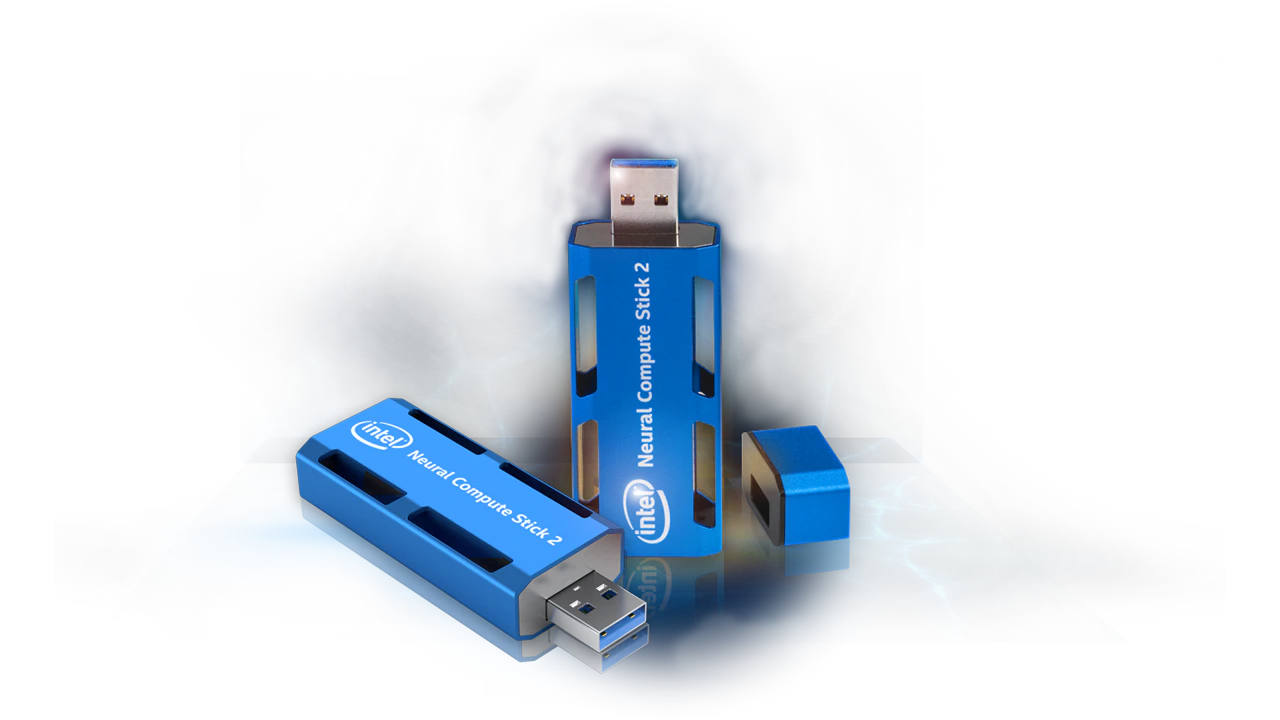
\includegraphics{obrazky-figures/ncs2.png}}
  \label{obrazek:ncs2}
  \caption{Intel Neural Compute Stick 2 \cite{ncs2}}
  \end{center}
\end{figure}

Experimenty provedené v~\cite{ncs2testYolo} porovnávají výkonnost akcelerátorů Nvidia Jetson Nano, Nvidia Jetson Xavier NX a Raspberry Pi 4B s~NCS2. K~porovnání posloužily frameworky YOLOv3 popsaný v~sekci \ref{sekce:NSdetektory} a YOLOv3--tiny. Experimenty byly založeny na detekci objektů ve dvou videích.
\begin{itemize}
  \item \emph{Video1} -- rozlišení 768 $\times$ 436 pixelů, celkem 1596 framů
  \item \emph{Video2} -- rozlišení 1920 $\times$ 1080 pixelů, celkem 960 framů 
\end{itemize}

Naměřené výsledky zobrazuje obrázek \ref{obrazek:ncs2test}.

\begin{figure}[H]
  \begin{center}
      \scalebox{0.5}{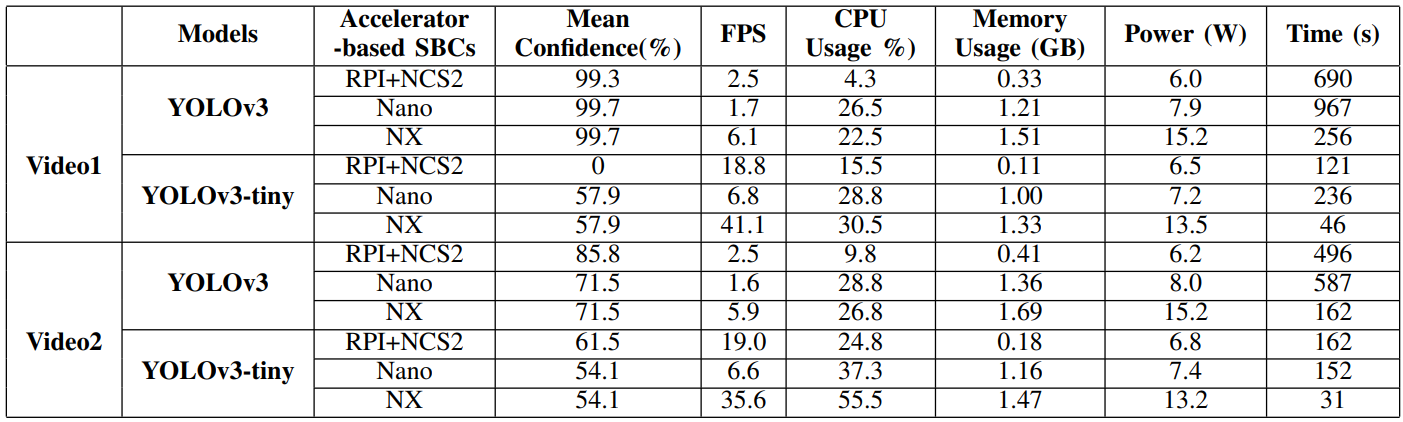
\includegraphics{obrazky-figures/ncs2test.png}}
  \label{obrazek:ncs2test}
  \caption{Výsledky testu akcelerátorů neuronovýxh sítí s~modelem YOLOv3 a~YOLOv3-tiny \cite{ncs2testYolo}}
  \end{center}
\end{figure}

Z~tabulky v~obrázku \ref{obrazek:ncs2test} můžeme vidět, že NCS2 dosahuje podobných výsledků detekce ve \emph{Videu1} jako Jetson Nano a zároveň nejméně zatěžuje procesor. U~\emph{Videa2} má NCS2 nejlepší výsledky detekce. Využití paměti s~větším vstupem roste, stále je však mezi konkurenty nejnižší, to samé lze řící o~spotřebě energie. S~dostatečně dobrým modelem neuronové sítě je tak NCS2 úsporným akcelerátorem s~vysokou úspěšností detekce.


\subsection*{OpenVINO}
Framework/knihovna OpenVINO se stará o~konverzi a optimalizaci natrénovaného modelu neuronové sítě v~jednom z~podporovaných frameworků (viz obrázek \ref{obrazek:ovchart}) pro použití na NCS2 nebo jiném zařízení (procesory, grafické karty). OpenVINO se nezaměřuje pouze na oblast počítačového vidění, ale na neuronové sítě obecně.

\begin{figure}[H]
  \begin{center}
      \scalebox{0.22}{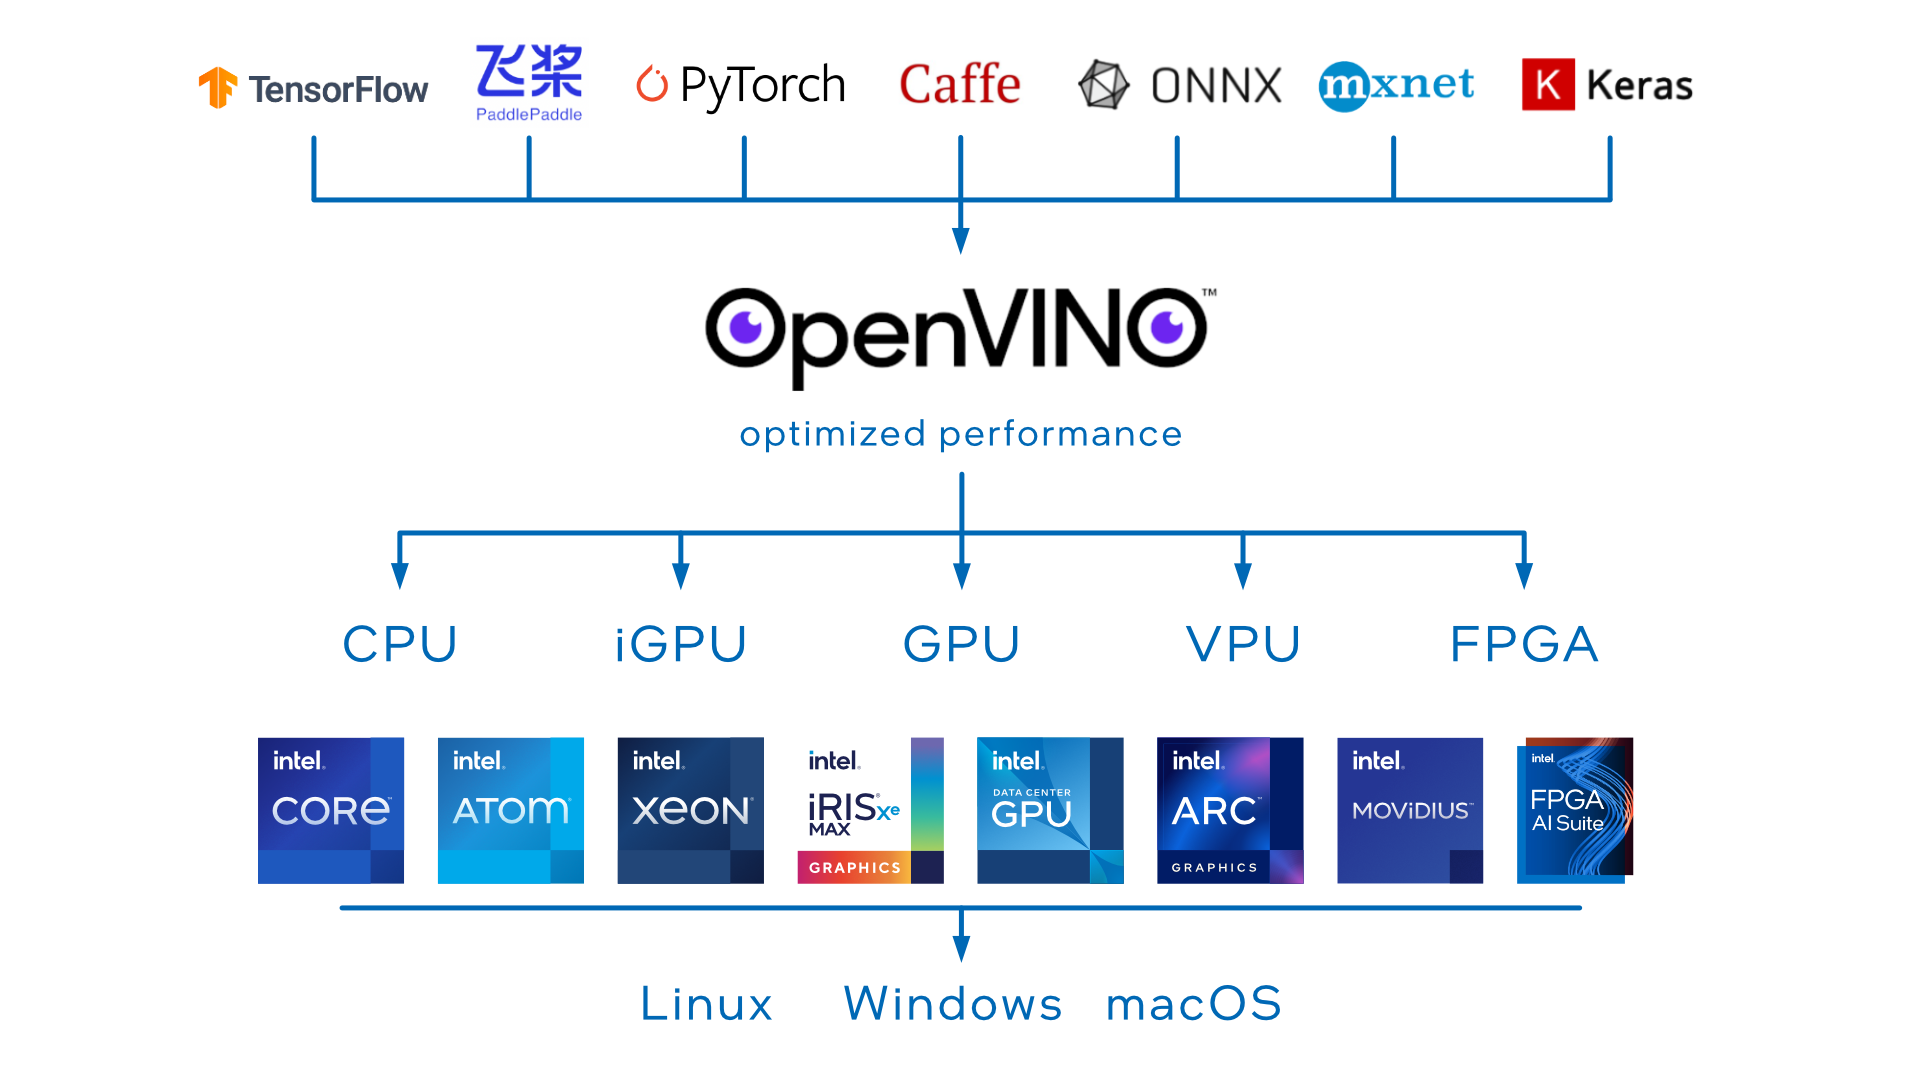
\includegraphics{obrazky-figures/ovchart.png}}
  \label{obrazek:ovchart}
  \caption{Využití frameworku OpenVINO \cite{openvino}}
  \end{center}
\end{figure}

%%%%%%%%%%%%%%%%%%%%%%%%%%%%%%%%%%%%%%%%%%%%%%%%%%%%%%%%%
%       KAPITOLA Návrh
%%%%%%%%%%%%%%%%%%%%%%%%%%%%%%%%%%%%%%%%%%%%%%%%%%%%%%%%%
\chapter{Návrh řešení}
Tato kapitola popisuje jak nástroje a postupy použité při realizaci řešení, tak také způsob získávání dat pro natrénování detekční neuronové sítě. Dále se kapitola zabývá návrhem této konvoluční neuronové sítě a návrhem způsobu získávání výsledků detekčních experimentů. V kapitole také nalezneme popis plán funkcí uživatelského rozhraní detektoru a přiblížení metody Mirnet.

\section{Použité nástroje}
\label{sekce:pouzite_nastroje}
K programování, akceleraci a vizualizaci výsledků detekce s využitím neuronových sítí je potřeba zvolit vhodný programovací jazyk, vhodné knihovny a frameworky. Mezi nejpoužívanější jazyky k tomuto účelu patří C++ a Python. Ze zadání byl vybrán jazyk Python. Tvorba neuronových sítí je usnadněna, pomocí k tomu určených knihoven jako jsou TensorFlow, PyTorch nebo ONNX. Akceleraci neuronových sítí na zařízeních značky Intel (tedy i NCS2) se věnuje knihovna OpenVINO. Aby bylo možné ověřit funkčnost detektoru, je potřeba grafické rozhraní pro zobrazování detekce. K tomuto účelu lze využít knihoven pro grafická uživatelská rozhraní jako jsou Tkinter nebo PyQt. Tato část vystihuje soubor zvolených nástrojů k vytvoření detektoru obličejů a možnostem jeho použití.

\subsection*{TensorFlow}
Framework \textbf{TensorFlow}, částečně popsaný v sekci \ref{sekce:frameworky_pro_ns}, slouží k programování aplikací strojového učení. Využívá knihovnu \textbf{Keras} a umožňuje vytvářet nebo používat existující modely neuronových sítí. Tvorba neuronových sítí je realizována spojováním různých vrstev sítě a nastavováním aktivačních funkcí, filtrů apod.
TensorFlow navíc poskytuje API pro různé aplikace umělé inteligence, jedno z těchto API se věnuje detekci objektů.\footnote{\url{https://github.com/tensorflow/models/blob/master/research/object_detection/g3doc/tf2_detection_zoo.md}}

V rámci frameworku TensorFlow je integrován program TensorBoard umožňující vizualizovat výsledky a průběh trénování a výsledky evaluace TensorFlow modelů.

\subsection*{OpenVINO}
Teoreticky je tato knihovna popsána v předcházející kapitole. Praktické použití knihovny spočívá ve využití části nazvané \textbf{Model Optimizer} sloužící k optimalizování modelu neuronové sítě pro dosažení nižší latence při zpracování obrázku při detekci. Model může být dále akcelerován pomocí kvantování hodnot vah jednotlivých vrstev neuronů. Knihovna zároveň funguje jako programové rozhraní pro práci s Intel Neural Compute Stick 2 a dalšími akcelerátory značky Intel.

\subsection*{PyQt6}
Knihovna PyQt6 je Python knihovna vycházející z C++ implementace grafické knihovy Qt6. Používá se k návrhu grafického uživatelského rozhraní aplikací napsaných v jazyce Python, pracuje se signály a sloty (události a jejich obsluha). Knihovna poskytuje rozhraní a třídy pro práci s více vlákny, umožňuje používat dialogová okna a je snadná na používání.


\section{Data}
\label{sekce:data_navrh}
Pro trénování neuronových sítí je potřeba mít dostatek trénovacích dat. Detektory obličejů jsou trénovány na obrázcích z datasetů, které musejí mít přidruženy anotační soubory se souřadnicemi poloh obličejů. V této sekci je popsán návrh vhodného datasetu a možnosti jeho rozšíření pomocí augmentace.

\subsection*{Datasety}
Mezi existujícími datasety obličejů lze v jednoduchosti nalézt dva druhy dat. Jedním druhem jsou takové datasety, které obsahují fotografie obličejů v poměru jeden obličej na jednu fotografii. Příkladem takového datasetu mohou být datasety \textbf{DigiFace1M} nebo \textbf{UTKFace} popsané v sekci \ref{sekce:datasety}. Tyto datasety mohou sloužit jako datasety k detekci obličejů, ale hodí se spíše na klasifikaci/rozpoznávání. Anotační soubory buď existují a obsahují souřadnice hranic obličeje na snímku, nebo úplně chybí a obrázek tak obsahuje pouze obličej -- souřadnice odpovídají rozměrům obrázku.

Druhou možností jsou datasety, kde je na jedné fotografii větší množství obličejů (případně je zde jen jeden obličej, ale nezabírá celou plochu obrázku). Tyto datasety mívají k daným obrázkům přidruženy anotační soubory, obsahující minimálně koordináty tváří, v případě některých (například \textbf{WIDER FACE}, zmíněný v sekci \ref{sekce:datasety}) jsou doplněny informace o rozmazání, póze, zastínění anebo zakrytí daného obličeje. Takovéto datasety jsou vhodné pro trénování detekčních neuronových sítí.

Body, udávající takzvané ohraničující boxy (anglicky \emph{bounding boxes}) v nichž se vyskytují tváře je možné zapsat v různých tvarech. Základní dělení je na tři typy zápisu těchto souřadnic: \textbf{Pascal VOC}, \textbf{COCO} a \textbf{YOLO} \cite{annotace_formaty}.

\textbf{PascalVOC} anotuje obličeje ve tvaru $x_{min}, y_{min}, x_{max}, y_{max}$, kde $x_{min}, y_{min}$ jsou souřadnice levého horního rohu a $x_{max}, y_{max}$ jsou souřadnice pravého dolního rohu ohraničení. Formát \textbf{COCO} využívá stejně jako PascalVOC hodnoty $x_{min}, y_{min}$ a přidává k nim údaje $width$ a $height$, odpovídající šířce a výšce hraničního obdélníku. Třetí z nejpoužívanějších stylů značení, \textbf{YOLO}, nahrazuje hodnoty $x_{min}, y_{min}$ hodnotami $x_{center}, y_{center}$, které značí střed ohraničení. Tento formát navíc stejně jako COCO poskytuje hodnoty $width$ a $height$, aby bylo možné určit celou plochu ohraničení. Graficky tyto formáty zobrazuje obrázek \ref{obrazek:annotace_formaty}.

\begin{figure}[H]
  \begin{center}
      \scalebox{0.33}{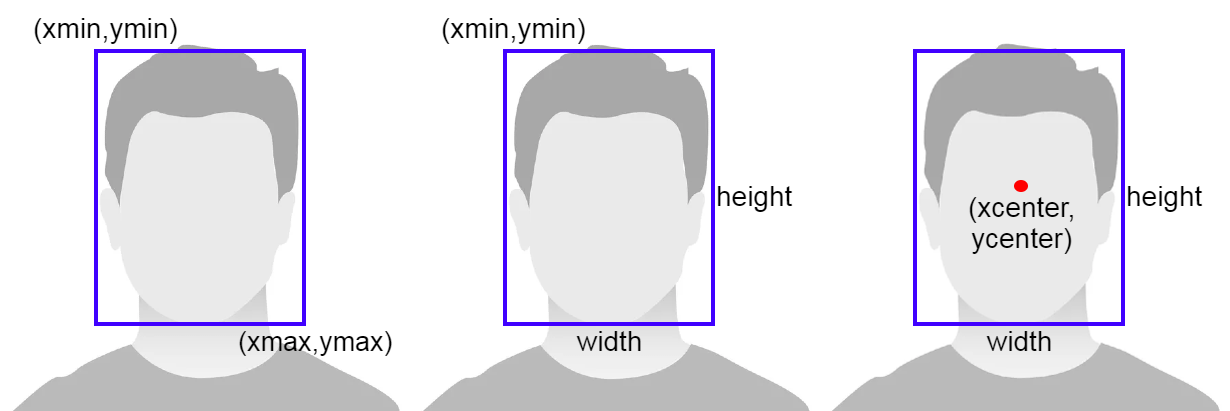
\includegraphics{obrazky-figures/annotation_formats.png}}
  \label{obrazek:annotace_formaty}
  \caption{Zobrazení anotací pomocí různých formátů. Zleva PascalVOC, COCO a YOLO}
  \end{center}
\end{figure}
 
\subsection*{Augmentace}
Dat z datasetů nemusí být vždy tolik, kolik je zapotřebí k natrénování dostatečně přesné neuronové sítě, nebo tyto data nemusejí přesně odpovídat zvolenému účelu a vytváření nových dat by bylo neefektivní. V těchto případech lze tento problém řešit augmentací.

Augmentace (s daty, jimiž jsou obrázky) spočívá v kopírování existujících dat s provedením různých úprav (jas, vystřižení části obrázu, otočení, kontrast, ISO, gamma, rozmazání, záměna barevných kanálů apod.). Takto nově vzniklá data pak lze použít jako dodatečná data k trénovacím obrázkům. Augmentaci lze provádět ručně, ale existují i specializované knihovny zajišťující, že v nově vzniklém obrázku budou automaticky vytvořeny anotační soubory se správně pozměněnými pozicemi obličejů.

\section{Detekční neuronová síť}
\label{sekce:detekcni_sit_navrh}
Neuronová síť pro detekci obličejů je, jak už bylo zmíněno výše, konvoluční neuronová síť, složená z několika různých vrstev (konvoluční vrstva, poolingová vrstva a další). Jelikož je detekční model často složen z velmi mnoha částí (např. generátor kotevních bodů/boxů -- anglicky \emph{anchor boxes}) a je náročné jej naprogramovat, poskytují frameworky pro práci s umělou inteligencí možnost využití API s předchystanými modely. Tyto modely pak je možno buď trénovat tzv. \uv{od nuly} nebo lze začít s trénováním částečně předtrénované sítě.

Při detekci ve zhoršených světelných podmínkách je vhodné využít některou z metod vylepšení obrázku (viz metody v sekci \ref{sekce:NSdetektory}). Jednou z nejlepších takovýchto metod je metoda Mirnet, tvořená natrénovanou neuronovou sítí, převádějící tmavé a špatně osvětlené obrázky na obrázky s lepší viditelností.

Tato sekce popisuje jak API pro detekci objektů z knihovny TensorFlow, tak detailně také metodu Mirnet.

\subsection*{TensorFlow 2 Object Detection API}
Framework TensorFlow poskytuje open\,--\,source API pro práci s modely pro detekci objektů\footnote{\url{https://github.com/tensorflow/models/tree/master/research/object_detection}} nebo například sledování (tracking) objektů. Toto API je podporováno TensorFlow verzí 1 i verzí 2 a umožňuje jednoduchým způsobem trénovat, validovat a testovat předpřipravené modely. Modely, které TensorFlow 2 Object Detection API (TF OD API) poskytuje jsou dostupné v tzv. TensorFlow 2 Detection Model Zoo. Tyto modely jsou předtrénovany na datasetu COCO 2017 a lze je tak využít na detekování jakýchkoliv objektů. Mezi nejznámější modely poskytované v rámci Detection Model Zoo patří \textbf{SSD ResNet50 V1 FPN} nebo \textbf{Faster R-CNN ResNet101}. Modely se liší mj. liší rozlišeními, s nimiž pracují, od 512 $\times$ 512 pixelů až po 1536 $\times$ 1536 pixelů.

TF OD API ke každému předtrénovanému modelu poskytuje základní informace o rychlosti detekce, o přesnosti změřené na validačních datech z výše zmíněného COCO datasetu a také informaci o tvaru výstupu neuronové sítě (souřadnice/klíčové body). Souřadnicový systém ohraničujích obdélníků odpovídá formátu PascalVOC. 

S modely se pracuje pomocí skriptů v jazyce Python (trénování, evaluace, export), nastavování se provádí skrze editaci konfiguračních souborů, které jsou poskytovány pro každý model zvlášť. Při trénování pak dochází k vytváření tzv. \emph{checkpointů}, vytvoření souborů s údaji o vahách neuronů. Trénování neprobíhá v epochách jak je tomu běžné, ale v krocích, kdy jeden krok znamená, že síť zpracuje počet obrázků daných velikostí \textbf{batch}. Z toho vyplývá nasledující vztah:

\begin{equation}
  \label{vzorec:krokuzaepochu}
  krokuZaEpochu = \frac{pocetObrazku}{batch}  \;\;[kroky]  
\end{equation}

\noindent Celkový počet proběhlých epoch pak lze vypočítat jako:

\begin{equation}
  \label{vzorec:celkemepoch}
  celkemEpoch = \frac{pocetKroku}{krokuZaEpochu}
\end{equation}


\subsection*{Mirnet}
Metoda Mirnet\cite{mirnet} je sofistikovaná metoda pro zlepšování kvality špatně osvětlených obrázků pomocí neuronové sítě. Metoda je tvořena několika bloky (Feature Extractor, Dual Attention Unit, Selective Kernel Feature Fusion a další), které postupně zpracovávají vstupní obrázek a snaží se jej zkvalitnit (zesvětlit, zvýraznit detaily). Architekturu Mirnetu zachycuje obrázek \ref{obrazek:mirnet}. Jelikož je Mirnet tvořen neuronovou sítí, je třeba jej před použitím natrénovat. K tomuto účelu je zapotřebí dataset s párovými obrázky, kdy oba obrázky zachycují stejný fenomén, ale na jednom z nich je snížená/zhoršená viditelnost (například tmou). Ideálním kandidátem na trénování, který splňuje tyto požadavky je dataset LoL Dataset\footnote{\url{https://daooshee.github.io/BMVC2018website/}} (ukázka viz obrázek \ref{obrazek:loldataset}). Dostatečně natrénovaná síť pak dokáže vylepšit vizuální kvalitu jakkéhokoliv obrázku, což je možno využít při detekci ve zhoršených světelných podmínkách.

\begin{figure}[H]
  \begin{center}
      \scalebox{0.45}{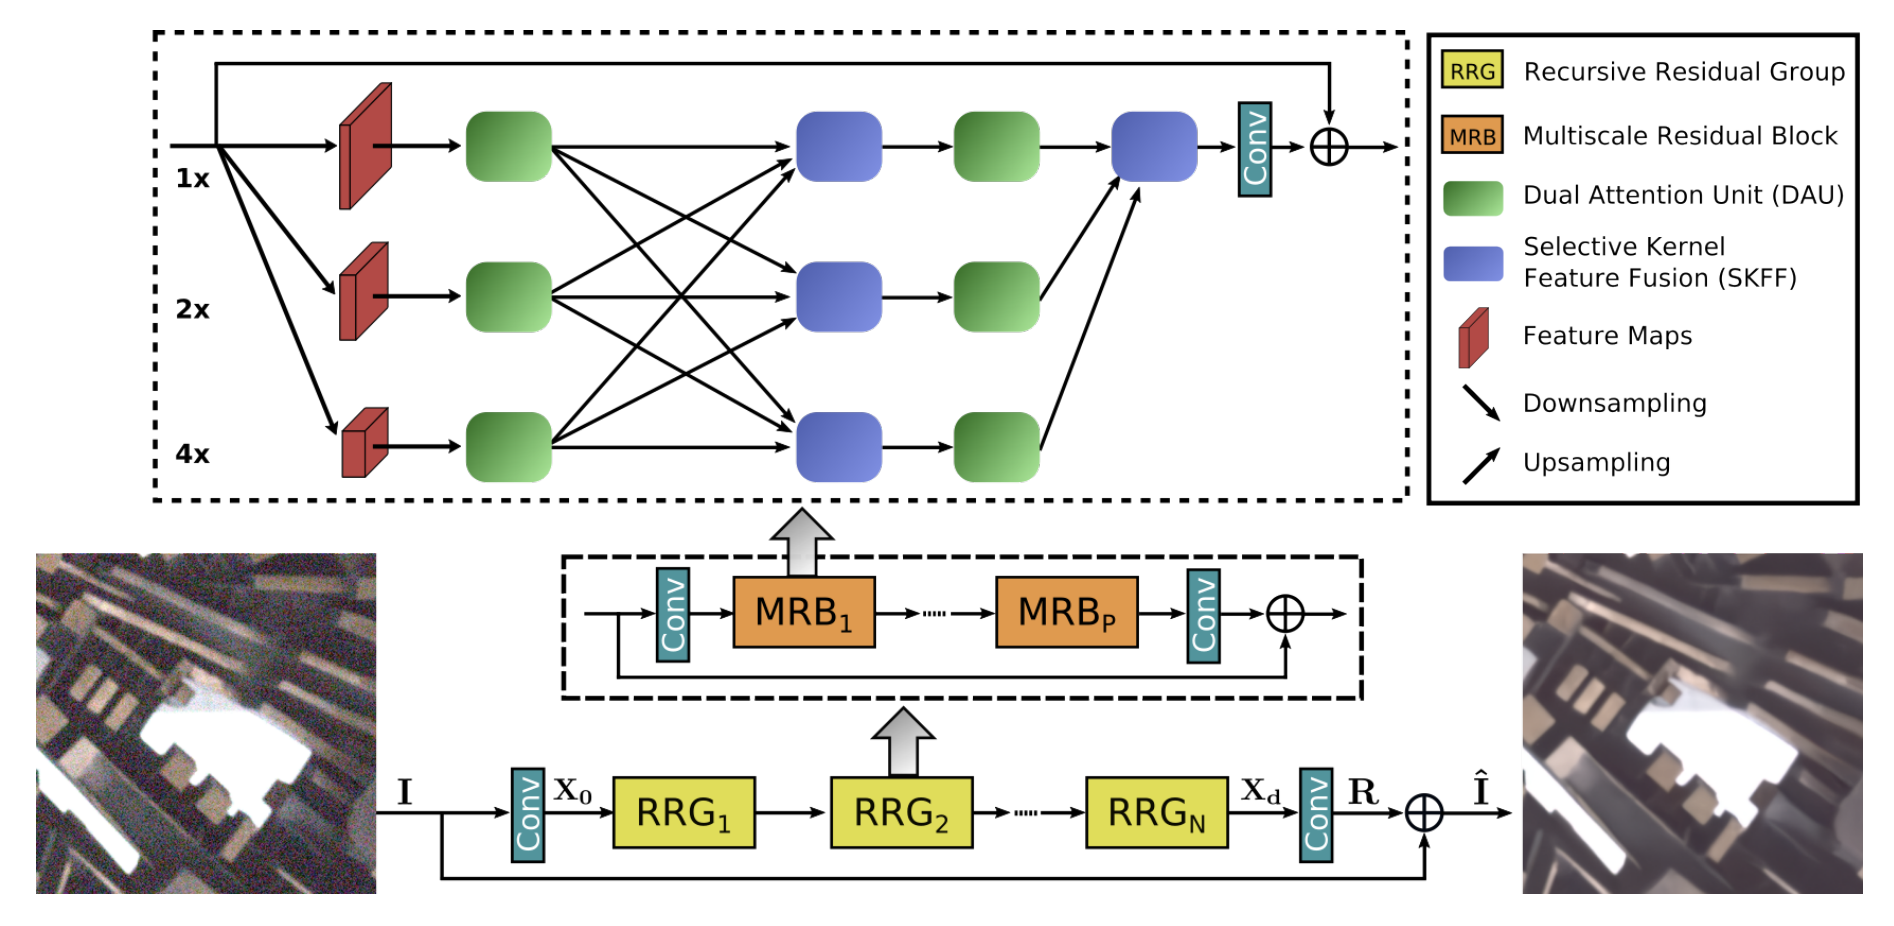
\includegraphics{obrazky-figures/mirnet_arch.png}}
  \label{obrazek:mirnet}
  \caption{Architektura neuronové sítě metody Mirnet}
  \end{center}
\end{figure}


\begin{figure}[H]
  \begin{center}
      \scalebox{0.35}{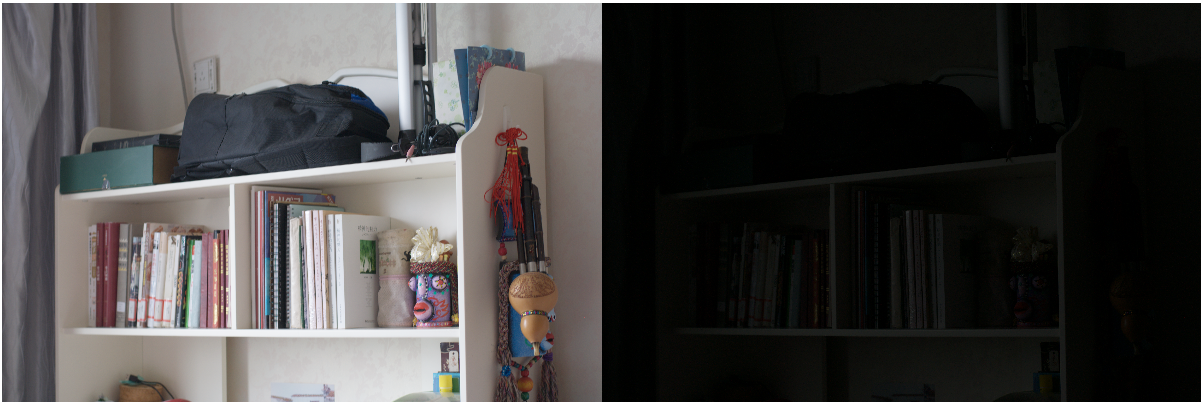
\includegraphics{obrazky-figures/loldataset.png}}
  \label{obrazek:loldataset}
  \caption{Ukázka párového snímku z datasetu LoL (vlevo normální snímek, vpravo stejný snímek se zhoršenou viditelností.)}
  \end{center}
\end{figure}
 
\section{Uživatelské rozhraní}
Výkonnost a úspěšnost detektorů může být vyhodnocována jednak veličinami přesnosti a rychlosti, ale také lidským pozorováním. Proto je vhodné detektory objektů používat ve spojení s grafickým uživatelským rozhraním, kdy jsou do promítaného videa nebo obrázku explicitně zakresleny lokátory detekovaných objektů, v tomto případě konkrétně tváří. Uživatelské rozhraní by ovšem mělo nejen umět přehrávat snímky a vykreslovat ohraničující obdélníky, ale také nabízet možnost kontroly přehrávání a možnost výběru vstupních dat. Nutnou součástí každého rozhraní pracujícího s videem by navíc měla být informace týkající se přehrávání -- aktuální čas a celková délka videa.

K návrhu grafického prostředí lze využít různorodé postupy, programy a knihovny. V rámci tvorby uživatelského rozhraní k této práci byla využita knihovna PyQt6 popsaná v sekci \ref{sekce:pouzite_nastroje}.

Aplikace navržená během tvorby této práce se však nestará jen o vyobrazení detekčních schopností navržené sítě, nýbrž také o přípravu dat pro vyhodnocení úspěšnosti a rychlosti detekce. Tato data (v případě úspěšnosti se jedná o procenta, v případě rychlosti pak o hodnotu FPS -- \emph{frames per second}, snímky za sekundu) finálně vyhodnocuje separátní program.

%%%%%%%%%%%%%%%%%%%%%%%%%%%%%%%%%%%%%%%%%%%%%%%%%%%%%%%%%
%       KAPITOLA Implementace
%%%%%%%%%%%%%%%%%%%%%%%%%%%%%%%%%%%%%%%%%%%%%%%%%%%%%%%%%
\chapter{Implementace}
\label{kapitola:implementace}
Předchozí kapitola pojednávala o návrhu nástrojů a postupů pro vytvoření detektoru obličejů ve zhoršených světelných podmínkách, tato kapitola navazuje líčením o implementaci těchto postupů. Na začátku implementace detekční sítě stojí příprava trénovacích dat (obrázků a anotačních souborů), popsaná v sekci \ref{sekce:priprava_dat}. Následně je nutné vybrat a implementovat neuronovou síť detektoru a natrénovat ji (viz sekce \ref{sekce:detektor_obliceju_implementace}). Pro zrychlení detekece je poté využito akceleračních nástrojů popsaných v předchozích kapitolách, v nynější kapitole se tomuto věnuje sekce \ref{sekce:akcelerace_implementace}. K experimentům je nezbytné implementovat grafické uživatelské rozhraní (sekce \ref{sekce:gui}) a příslušné vyhodnocovací nástroje a programy (viz sekce \ref{sekce:nastroje_pro_experimenty}).

\section{Příprava dat}
\label{sekce:priprava_dat}
Tématem této frakce je příprava fotografií z datasetů k trénování neuronové sítě. Proces předchystání dat spočívá ve zvolení vhodného datasetu pro detekci obličejů, anotováním obličejů ve fotografií (pokud toto není dostupné přímo s datasetem) a provedením augmentace za účelem znásobení počtu dat a provedení případných úprav pro konkrétní zadání (v tomto případě mj. ztmavení). Konečným bodem přípravy je převod dat do TensorFlow formátu \textbf{TFRecords}. Takto nachystané prostředky pak lze použít k trénování.

\subsection*{Použité datasety}
Pro detekci obličejů bylo zásadní zvolit vhodný dataset. V průběhu práce byly zvažovány a zkoušeny různé datasety a nakonec bylo rozhodnuto, že budou použity 2 datasety. Konkrétně dataset WIDER FACE a dataset DARK FACE, oba uvedené v sekci \ref{sekce:datasety}.

WIDER FACE poskytuje k trénovacím a validačním obrázkům anotační soubory v anotačním formátu COCO (viz sekce \ref{sekce:data_navrh}). Trénovacích souborů je dostupných celkem 12880, z nichž bylo odebrány ty, na nichž se nevyskytují žádné obličeje. Z takto filtrovaného výběru potom bylo vzato prvních 12000 snímků a byla provedena augmentace.

\begin{figure}[H]
  \begin{center}
      \scalebox{0.35}{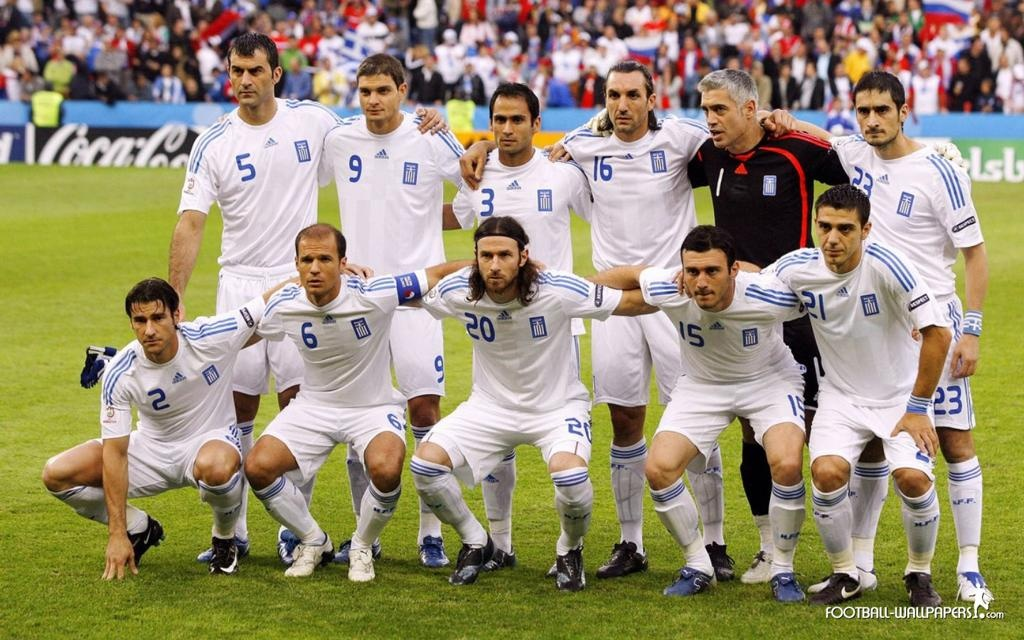
\includegraphics{obrazky-figures/widerface_example.jpg}}
  \label{obrazek:widerfaceexample}
  \caption{Ukázka snímku z datasetu WIDER FACE}
  \end{center}
\end{figure}

DARK FACE dataset dává k dispozici 6000 anotovaných obrázků vyfocených v noci v městském prostředí (viz ukázka na obrázku \ref{obrazek:darkfaceexample}). Z těchto 6000 fotek bylo prvních 4800 vybráno jako trénovací data (zbytek byl využit jako validační dataset). Následně byla provedena augmentace, podobně jako s datasetem WIDER FACE.

\begin{figure}[H]
  \begin{center}
      \scalebox{0.35}{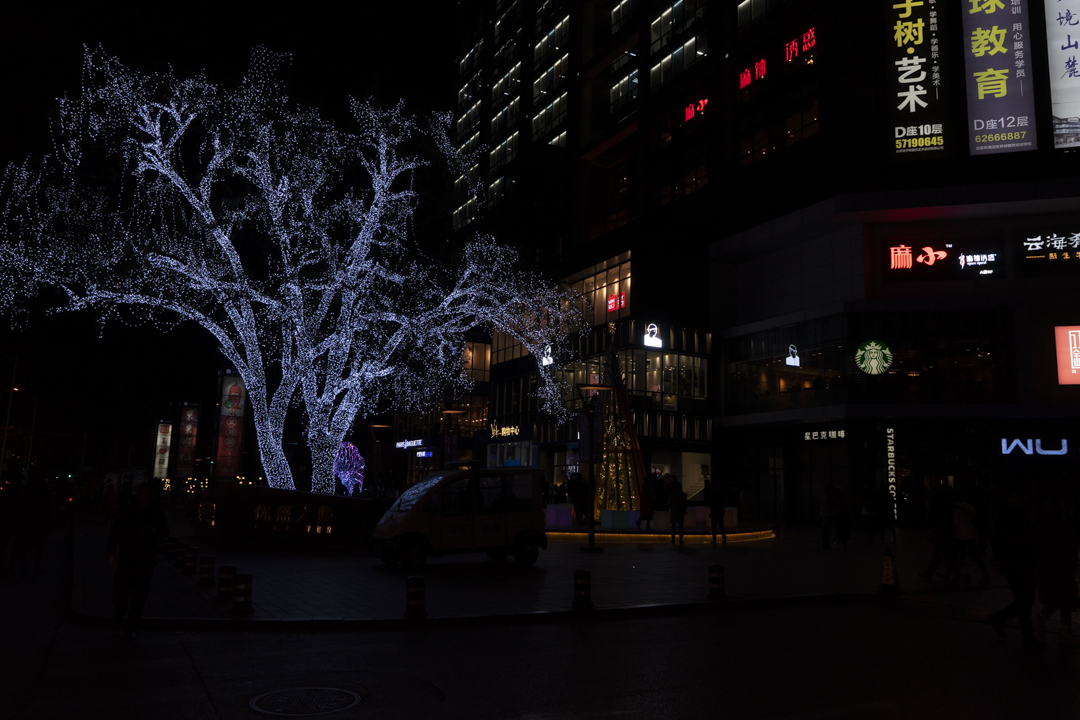
\includegraphics{obrazky-figures/darkfaceexample.png}}
  \label{obrazek:darkfaceexample}
  \caption{Ukázka snímku z datasetu DARK FACE}
  \end{center}
\end{figure}

\subsection*{Augmentace fotografií WIDER FACE}
Obecně byla augmentace rozebrána v sekci \ref{sekce:data_navrh}, konkrétně se v práci k provedení augmentace používá Python knihovna \textbf{albumentations}. Proces augmentace sestává z několika kroků. Prvním z nich
je zisk anotačních dat z anotačního souboru. První údaj obsahuje název fotografie, za ním následuje číslo udávající počet obličejů v obrázku a poté hraniční body všech obličejů v daném snímku.

Poté následuje načtení originální fotografie z datasetu WIDER FACE do augmentačního programu. Na načtené fotografii je provedena augmentace -- je vytvořena kopie, v níž jsou s určitou pravděpodobností (viz číslo v závorce) provedeny tyto úpravy:

\begin{itemize}
  \item horizontální převrácení (0.5),
  \item vertikální převrácení (0.5),
  \item náhodná změna jasu a kontrastu směrem ke ztmavení (0.7),
  \item náhodná změna gammy (0.1),
  \item přidání Gaussova šumu (0.2),
  \item přidání ISO šumu (0.4).
\end{itemize}

Pro vytvořený augmentovaný obrázek (ukázka na obrázku \ref{obrazek:augmentovanyobrazek}, originál viz obrázek \ref{obrazek:widerfaceexample}) přepočítá knihovna albumentations nové souřadnice obličejů. Obrázek je pak uložen a anotační data skládající se z \textbf{názvu obrázku}, \textbf{souřadnic obličejů ve formátu PascalVOC} a \textbf{klasifikačních tříd} (všechny objekty patří do třídy \emph{face}), jsou uložena ve formátu JSON. Podobný anotační JSON soubor se vytvoří i pro originální fotografii. Názvy obrázků jsou při tomto procesu nastaveny na číselné hodnoty 1.jpg až 12000.jpg pro originální snímky a na hodnoty 1.0.jpg až 12000.0.jpg pro augmentované obrázky. Celkem je tak k trénování připraveno 24000 obrázků.

\begin{figure}[H]
  \begin{center}
      \scalebox{0.35}{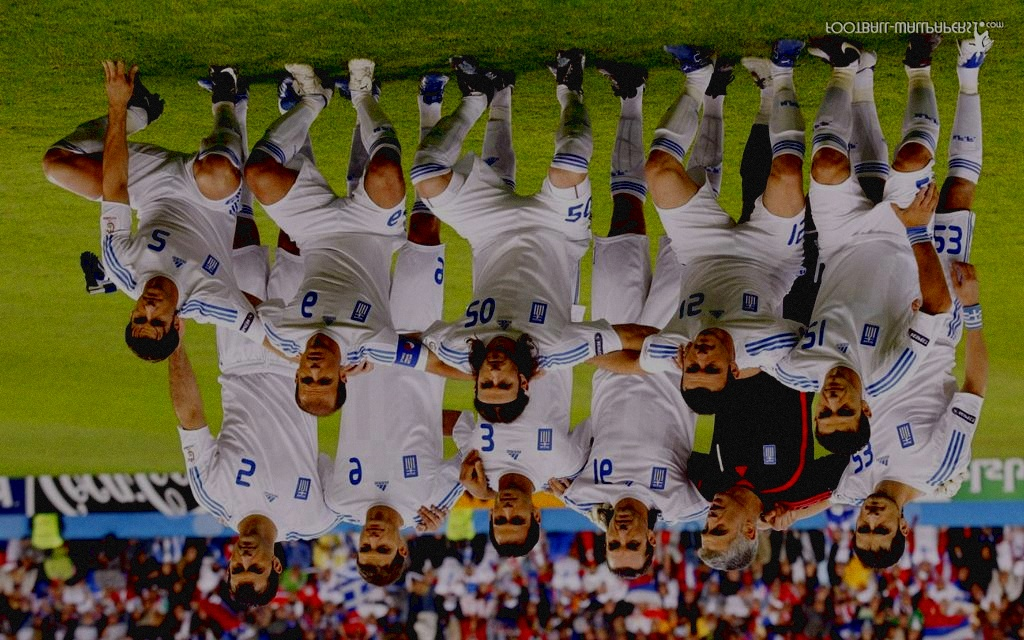
\includegraphics{obrazky-figures/augmentedexample.jpg}}
  \label{obrazek:augmentovanyobrazek}
  \caption{Ukázka augmentovaného snímku z datasetu WIDER FACE}
  \end{center}
\end{figure}

\subsection*{Augmentace fotografií DARK FACE}
Augmentace obrázků z datasetu DARK FACE je velmi podobná augmentaci fotografií z datasetu WIDER FACE. Anotační soubor zda má mírně odlišnou syntaxi a výčet úprav je ochuzen o Gaussův šum a snížení pravděpodobnosti změny jasu a kontrastu na 0.5. Výstup augmentačního skriptu ovšem zachovává stejný formát. S využitím augmentace je tak vytvořeno 4800 nových snímků (1.0.png až 4800.0.png) a celkem tak trénovací set tvoří 9600 tmavých obrázků.

\subsection*{TFRecord}
Vstupy TensorFlow modelů neuronových sítí mohou být dvojice dat vstup $\times$ výstup nebo se může jednat o serializovanou strukturu dat formátu \textbf{tfrecord}\footnote{\url{https://www.tensorflow.org/tutorials/load_data/tfrecord}}. Jedná se o binární sekvenci dat, mající určitou organizaci a řád. Výhodou použití tfrecord namísto klasických obrázků a anotačních souborů je to, že odpadá část předzpracování dat před spuštěním trénování sítě. Skript starající se o transformaci originálních a augmentovaných obrázků a popisných souborů do formátu tfrecord pracuje tak, že načte obrázek a anotační soubor a provede kontrolu, že žádný ohraničující box nezasahuje mimo rozměry obrázku. Dále pak vytvoří proměnnou typu \texttt{tf.train.Example}, která tvoří základ jednoho tfrecordu. Do proměnné se zapisují bytová data dle následujícího řádu:

\begin{itemize}
  \item data obrázku,
  \item výška,
  \item šířka,
  \item název obrázku,
  \item formát obrázku,
  \item ID obrázku (odpovídá názvu),
  \item PascalVOC formát pozice obličeje,
  \item název a číslo třídy objektu (1 a \uv{face}).
\end{itemize}

Z důvodu snazší manipulace s daty ve formátu tfrecord byly obrázky z datasetu WIDER FACE rozděleny do skupin po 2000 jednotkách. Celkově tak bylo vytvořeno 12 trénovacích tfrecord souborů (12000 originálních a 12000 augmentovaných obrázků po dvoutísícových skupinách). Pro druhý dataset byly vytvořeny skupiny po 200 snímcích a vzniklo tak 48 tfrecord souborů.

\section{Detektor obličejů}
\label{sekce:detektor_obliceju_implementace}
Tato část pojednává o implementaci použitého detektoru obličejů. Zabývá se návrhem a tvorbou původního modelu pro detekci a následně i použitím konkrétních zvolených existujících modelů. V původním plánu byla snaha o vytvoření plně vlastního detektoru obličejů, od čehož bylo upuštěno pro příliš vysokou náročnost. Tomuto prvotnímu záměru se věnuje první část této sekce. Přirozeně pak následujícím krokem byl přechod na modely existující. K tomuto účel bylo vybráno TensorFlow Object Detection API (TF OD API) popsané v sekci \ref{sekce:detekcni_sit_navrh}. Výsledný detektor, respektive detektory tváří tak stojí na základech detektorů objektů. Explicitně využité modely neuronových sítí popisují další pasáže této sekce.

\subsection*{Původní záměr}
Jak již bylo avizováno výše, původní záměr spočíval ve vytvoření vlastní detekční sítě s využitím frameworků TensorFlow a Keras. Po několika pokusech se podařilo vytvořit a natrénovat model podobný neuronové síti VGG--16. Tento model zvládal detekovat pouze 1 obličej, protože se spíše než o detektor jednalo o klasifikátor (který klasifikoval v obrázku obličej a dokázal vrátit souřadnice ohraničení tváře). Následným testováním na obrázcích s více obličeji, kdy bylo vyzkoušeno oblast detekovaného obličeje v obrázku začernit a pokusit se o detekci znovu, bylo zjištěno, že metoda je neefektivní a nepříliš funkční.

Novým způsobem, který bylo možné zkusit zrealizovat byla celková implementace SSD detektoru. Poměrně složité matematické operace s jednotlivými vrstvami výstupů detekční sítě se ukázaly být příliš náročné na implementaci. Bylo tak rozhodnuto, o využití existujícího řešení s implementací vlastní augmentace vstupních dat a vlastního natrénování. Při trénování muselo být využito dostupného předtrénovaného stavu sítě, protože kompletní trénování sítě tzv \uv{od nuly} by zabralo neúnosně mnoho výpočetního i reálného času.

Použité modely tak vycházejí z detektorů objektů a jsou přetrénovány tak, aby detekovaly jen 1 třídu objektů (obličeje), místo výchozích 90 tříd. V tom se také odlišují od konkrétně zaměřených detektorů tváří jako je například RetinaFace, která byla trénována přímo pro detekci obličejů.

\subsection*{SSD ResNet50 V1 FPN}
Prvním zvoleným modelem z TensorFlow 2 Detection Model Zoo\footnote{\url{https://github.com/tensorflow/models/blob/master/research/object_detection/g3doc/tf2_detection_zoo.md}} (TF DMZ) byl model SSD ResNet50 V1 FPN 640x640 (RetinaNet50). Jak název napovídá, jedná se o neuronovou síť ResNet50 spojenou s kaskádou SSD. Model má na vstupu preprocessingovou část, která se stará o změnu rozlišení vstupního obrázku na 640 $\times$ 640 pixelů. Dle stránek TF DMZ dosahuje ve výchozím předtrénovaném stavu model rychlosti detekce 46 ms a má průměrnou přesnost 34,3 \% na datasetu COCO 2017.

SSD část tohoto modelu je popsána v sekci \ref{sekce:NSdetektory}. Síť ResNet50 (Residual Network) \cite{resnet} je konvoluční neuronová síť patřící mezi skupinu ResNet modelů, mající 50 vrstev. Vychází z původního 18, respektive 34 vrstvého ResNetu. Každá vrstva obsahuje konvoluční filtr 3 $\times$ 3. Konkurentem ResNetu je například síť VGG--16. Další verze ResNetu mají 101 nebo 152 konvolučních vrstev.

Tento model byl natrénován na datasetech popsaných výše. Samotné trénování popisuje sekce \ref{sekce:trenovani}. Po natrénování byl model vyzkoušen při detekci. Bez konkrétního měření přesnosti (konkrétní hodnoty byly změřeny později a jsou zaznamenány v experimentech v kapitole \ref{kapitola:experimenty}) dosahoval model obstojných výsledků detekce obličejů, ovšem ukázalo se, že detekce je pomalá a nelze s ním detekovat tváře ve videu v reálném čase. Proto byl hledán jiný, rychlejší model a nakonec byl ustanoven model SSD MobileNet V2 FPNLite.

\subsection*{SSD MobileNet V2 FPNLite}
SSD MobileNet V2 FPNLite 640 $\times$ 640 je model složený z SSD části a neuronové sítě MobileNet. MobileNet \cite{mobilenet} je pro svou efektivitu a rychlost určen převážně pro mobilní zařízení (například v Android telefonech jej lze použít s TensorFlow Lite), ale může posloužit i jako real--time detektor na běžném počítači. MobileNet používá stejně jak ostatní  detekční sítě konvoluční vrstvy, ale konvoluce v něm je rozdělena na tzv \emph{depthwise} a \emph{pointwise} část. Depthwise konvoluce je aplikována na každý vstupní kanál a pointwise konvoluce pak na tento výstup aplikuje konvoluci s filtrem o velikosti 1 $\times$ 1. Velikost sítě v počtu vrstev je poloviční oproti ResNet50. Velikost na disku je v případě MobileNetu 10$\times$ nižší než v případě ResNet50.

MobileNet podle dat z TF DMZ dosahuje rychlosti zpracování 1 obrázku za 39 ms a průměrná úspěšnost na datasetu COCO 2017 je 28,2 \%. Model stejně jako předcházející ResNet50 pracuje s rozlišením 640 $\times$ 640 pixelů. V práci byly nakonec použity oba modely a během experimentů byly porovnány mezi sebou.

\section{Trénování}
\label{sekce:trenovani}
Následující blok je věnován problematice trénování vybraných neuronových sítí z předcházející sekce. Neboť je trénování detekčních neuronových sítí velmi výpočetně a časově náročná akce, je potřeba mít výkonnou grafickou kartu nebo využít trénování v cloudu (například Google Colab). Autor textu nejprve zkoušel trénovat síť na vlastní grafické kartě nVidia GTX 1070 Ti s 8 GB video paměti RAM. To se ukázalo jako příliš pomalé a tak bylo trénování přesunuto na servery služby Metacetrum. Podrobněji Metacentrum popisuje text níže.

\subsection*{Metacentrum}
Metacentrum je virtuální organizace spravovaná organizací Cesnet, která poskytuje zdarma akademickým pracovníkům a studentům vypočetní zdroje na několika serverech po celé ČR. Spouštění úloh je realizováno interaktivě nebo dávkově. Pro potřeby trénování bylo využito dávkových úloh, které spočívají v přípravě bash skriptu a jeho následném předání plánovači úloh. Skripty dávkových úloh mají danou počáteční syntaxi dle pravidel Metacentra (nastavení požadovaných zdrojů, požadovaná délka běhu atd.). Po těcto pravidlech následuje klasický kód v bashi.

Aby mohlo trénování běžet, bylo potřeba předpřipravit prostředí na serverech Metacentra. Příprava sestávala z vytvoření virtuálního prostředí (pomocí aplikace micromamba) pro běh TF OD API, samotná instalace TF OD API a instalace potřebných knihoven pro práci s grafickými kartami nVidia (cuDNN 8.1.0 a CUDA 11.2). Pro trénování pak byl vybrán téměř vždy server Galdor s využitím dvou grafických karet nVidia A40.

Trénink modelu z TF OD API se spouští speciálním Python skriptem, který je obsažen v repozitáři TF OD API. Skript ke spuštění potřebuje znát místo uložení trénovaného modelu a také konfigurační soubor \texttt{pipeline.config}. V tomto konfiguračním souboru se nastavují parametry trénování (optimizér, počet kroků, batch velikost, míra učení -- \emph{learning rate}, maximální počet detekcí v obrázku, počet detekovaných tříd, druhy a váhy jednotlivých chybových funkcí a další parametry) a také místo uložení trénovacích a evaluačních TFRecord souborů a lokace výchozího předtrénovaného bodu modelu.

Skript pro učení modelu automaticky každých 1000 provedených kroků ukládá aktuální stav modelu do tzv. checkpointů. Tyto checkpointy je pak možno převést na klasický TensorFlow \emph{saved model} formát a následně použít k detekci. Výstupní hodnoty jednotlivých chybových funkcí jsou při běhu trénování vypisovány na standardní chybový výstup ve formátu, který zachycuje obrázek \ref{obrazek:trenovani}.

\begin{figure}[H]
  \begin{center}
      \scalebox{0.7}{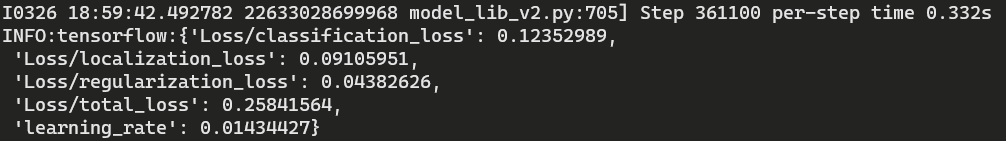
\includegraphics{obrazky-figures/trenink.png}}
  \label{obrazek:trenovani}
  \caption{Výstup trénovacího skriptu během trénování}
  \end{center}
\end{figure}

\subsection*{Natrénované modely}
Celkově byly natrénovány 4 modely. Oba modely popsané v sekci \ref{sekce:detektor_obliceju_implementace} s oběma datasety ze sekce \ref{sekce:priprava_dat}. Jednotlivé parametry trénovaných modelů zachycuje tabulka \ref{tabulka:trenovanimodely}. Zkratky  DF a WF v názvech modelů odpovídají názvu datasetu, který byl použit při tréninku (DF = DARK FACE, WF = WIDER FACE). Počet kroků je metrika, kterou používá k počítání průběhu trénování TF OD API. Počet epoch je pak vypočítán dle vzorce \ref{vzorec:celkemepoch}. Velikost batche byla nastavena na hodnotu 32 z toho důvodu, aby nedocházelo při trénování k problémům s nedostatkem video paměti. Počty trénovacích obrázků odpovídají velikostem augmentovaným datasetům, které byly popsány výše.

\begin{table}[h]
  \begin{tabular}{|c|c|c|c|c|c|}
    \hline
    \rowcolor[HTML]{E0DBDB} 
    {\color[HTML]{333333} \textbf{Model}} & {\color[HTML]{333333} \textbf{Kroků}} & {\color[HTML]{333333} \textbf{Epoch}} & {\color[HTML]{333333} \textbf{Doba trénování}} & {\color[HTML]{333333} \textbf{Batch}} & {\color[HTML]{333333} \textbf{Počet tr. obrázků}} \\ \hline
    DF Mobilenet  & 100 000 & $\sim$333 & 5,5 h  & 32  & 9 600        \\ \hline
    DF Resnet50  & 500 000  & $\sim$1667   & 4 dny  & 32  & 9 600   \\ \hline
    WF Mobilenet    & 362 000      & $\sim$483 & 40 h   & 32  & 24 000  \\ \hline
    WF Resnet50   & 500 000  & $\sim$667  & 3,5 dnů   & 32  & 24 000  \\ \hline
  \end{tabular}
  \label{tabulka:trenovanimodely}
  \caption{Parametry modelů natrénovaných v rámci práce}
\end{table}

Checkpointy, které trénováním vznikly pak byly pomocí TF OD API převedeny exportérem na tzv \emph{saved model} formát. Tento formát je klasický TensorFlow formát modelů, jenž se dá v dalších aplikacích načíst a použít k detekci.

\subsection*{Mirnet}
Poněvadž je práce zaměřena na detekci ve zhoršených světelných podmínkách a využívá metodu Mirnet, která je sama neuronovou sítí, bylo třeba natrénovat i ji. K tomuto účelu postačila vlastní grafická karta autora a nebylo třeba využívat služeb Metacentra. Kód neuronové sítě Mirnetu byl převzat z \cite{mirnet}. Trénování sítě bylo spuštěno po dobu 70 epoch a byl použit dataset LoL. 350 obrázků z tohoto datasetu bylo využito k trénování a zbylých 135 pak k validaci modelu. Vzhledem k vysoké náročnosti na video paměť, byl batch nastaven na velikost 1. 



\section{Akcelerace detekce}
\label{sekce:akcelerace_implementace}
Teorie věnující se akceleraci neuronových sítí a akcelerační knihovně OpenVINO byla shrnuta v sekci \ref{sekce:akcelerace}. Tato část je zaměřena na konkrétní implementaci a použití knihovny OpenVINO během práce na detektoru obličejů. Samotné detekční modely vytvořené s pomocí frameworku TensorFlow, které byly popsány výše, nedosahují na málo výkonném hardwaru požadované rychlosti zpracování vstupního videa. Řešením je použití akcelerační knihovny, která inferenci modelu výrazně urychlí, lze ji však využít jen na hardwaru značky Intel.

Akcelerace provedená v rámci této práce stojí na dvou pilířích z knihovny OpenVINO -- Model Optimizer a kvantování. \textbf{Model Optimizer} je vstupním bodem v práci s knihovnou OpenVINO. Stará se o převedení uloženého TensorFlow modelu do formátů XML a BIN. Další možností ještě vyšší akcelerace je tzv. \textbf{kvantování}, které nemusí být dostupné a funkční na každém Intel zařízení. Kvantování však umožňuje razantní nárůst rychlosti se zanedbatelným vlivem na přesnost detekce. Obě tyto činnosti jsou shrnuty na následujících řádcích.

\subsection*{Model Optimizer}
Utilita \textbf{Model Optimizer}\footnote{\url{https://docs.openvino.ai/latest/openvino_docs_MO_DG_Deep_Learning_Model_Optimizer_DevGuide.html}} se stará o převod a přizpůsobení modelu pro práci s možnostmi knihovny OpenVINO. Optimizer je součástí knihovního balíčku a spouští se jako samostatný program v příkazovém řádku. Typický pracovní postup Model Optimizeru zachycuje obrázek \ref{obrazek:moworkflow}. Jak již bylo zmíněno, program vytváří 2 soubory -- XML a BIN. XML soubor uchovává topologii neuronové sítě a v BIN souboru jsou uloženy váhy a biasy natrénované sítě.

\begin{figure}[H]
  \begin{center}
      \scalebox{0.5}{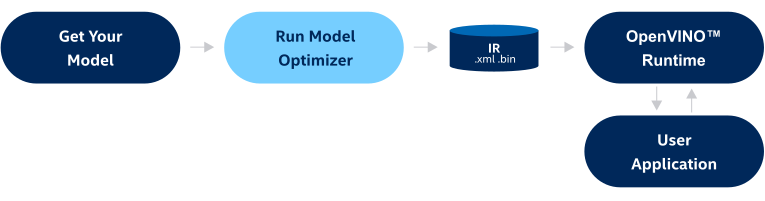
\includegraphics{obrazky-figures/moworkflow.png}}
  \label{obrazek:moworkflow}
  \caption{Postup použití (workflow) Model Optimizeru}
  \end{center}
\end{figure}

Při převodu obyčejného TensorFlow nebo PyTorch modelu stačí programu předat cestu k uloženému modelu. Transformace modelu z TensorFlow Object Detection API (TF OD API) je nicméně o něco složitější. Model Optimizeru musí být předána cesta k uloženému modelu (parametr \texttt{saved\_model\_dir}), dále pak cesta ke konfiguračnímu souboru modelu (\texttt{tensorflow\_object\_detection\_api\_pipeline\_config}) a také lokace tzv. transformačního konfiguračního souboru (\texttt{transformations\_config}), který je specifický pro modely z TF OD API.

Aby byla co nejvíce navýšena rychlost detekce na Intel Neural Compute Stick 2 (NCS2), byl navíc přidán parametr \texttt{data\_type} s hodnotou FP16. Ten zajistí, že model bude po převodu používat jen 16bitový float systém, což by mělo vést k celkovému zvýšení rychlosti inference. Posledním parametrem použitým při převodu je \texttt{input\_shape}, nastavující vstup detektoru na 640 $\times$ 640 pixelů.

Transformovaný model pak dosahuje značného zrychlení jak ukazují experimenty v kapitole \ref{kapitola:experimenty}. Akceleraci však lze ještě vylepšit pomocí kvantování.

\subsection*{Kvantování}
Kvantování \cite{quantization} pomocí knihovny OpenVINO je proces, při němž dochází k transformaci modelu z floating point aritmetiky na 8 bitovou celočíselnou aritmetiku. Model se tak stává více \emph{HW--friendly} a může tak běžet rychleji. Zároveň nedochází k rapidnímu snížení výkonnosti detekce.

Základní princip při kvantování zobrazuje obrázek \ref{obrazek:kvantovani}. Model neuronové sítě převedený OpenVINO Model Optimizerem, který pracuje s 32bitovými nebo 16bitovými floaty je kvantován, tak aby využíval 8 bitová velá čísla na interní výpočty modelu. Na výstupu jsou pak celá čísla převedena zpět na floaty. 

\begin{figure}[H]
  \begin{center}
      \scalebox{0.5}{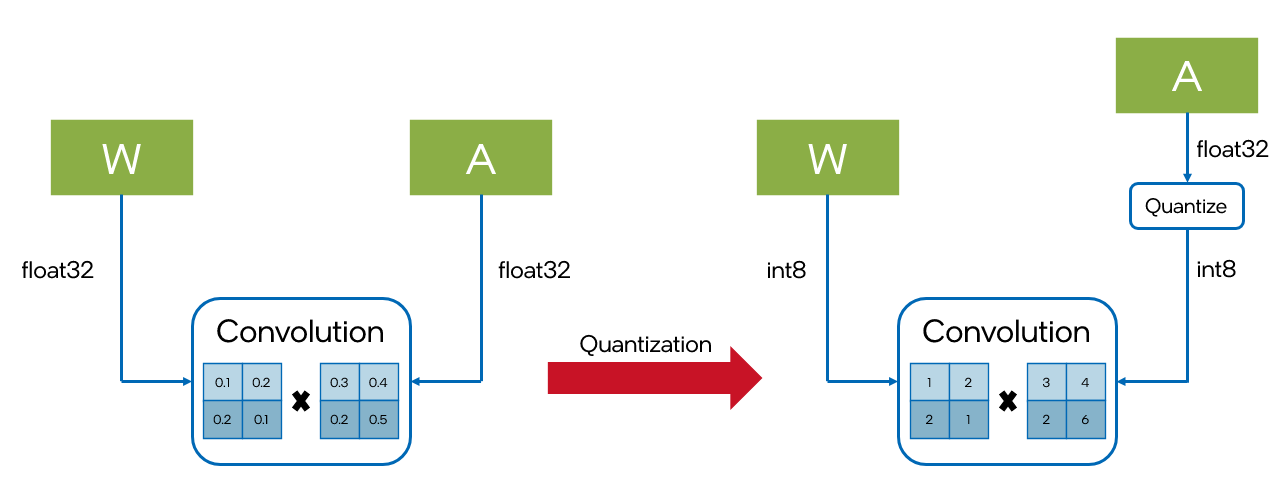
\includegraphics{obrazky-figures/kvantovani.png}}
  \label{obrazek:kvantovani}
  \caption{Ukázka principu kvantování neuronových modelů \cite{quantization}}
  \end{center}
\end{figure}

Skript starající se o kvantování modelů používaných v rámci této práce, potřebuje na vstupu kromě XML a BIN souborů modelu také kalibrační dataset. Dle dokumentace by tento dataset měl být tvořen snímky z trénovacího nebo validačního balíčku a obsahovat alespoň 300 fotografií. Kvantování pak probíhá za spolupráce knihovny \textbf{nncf} a OpenVINO, výstupní model je uložen opět ve formátu XML a BIN souborů. Vliv kvantování na rychlost lze posoudit z grafů v kapitole \ref{kapitola:experimenty}. Nevýhodou kvantování je mj. to, že takto pozměněný model nelze spustit na NCS2, které s celými čísly neumí pracovat. Kvantování již z logiky věci zmenšuje celkovou velikost modelu.

\section{Grafické uživatelské rozhraní}
\label{sekce:gui}
Grafické uživatelské rozhraní (GUI) aplikace vytvořené k praktickému zkoušení modelů bylo vytvořeno tak, aby nejen zobrazovalo video a detekované obličeje, ale také tak, aby umožňovalo vytvářet soubory s naměřenými metrikami pro další zpracování. Funkce a schopnosti GUI, způsoby měření, provádění detekce a organizaci výstupů jsou shrnuty v následujím oddílu. 

\subsection*{Rozhraní}
Kostra aplikace je postavena na knihovně PyQt6 a jejích signálech a slotech (události a reakce na ně). Rozhraní (viz obrázek \ref{obrazek:gui}) se skládá z několika sekcí. Horní část slouží k výběru přehrávaného videa ve formátu mp4 a výběru modelu pro detekci (jeden ze čtyř natrénovaných z předcházející části). Dále lze pak vybrat zařízení na němž detekce poběží v případě spuštění akcelerované OpenVINO verze modelu (NCS2, CPU, GPU), a nakonec je možno určit zda se má použít akcelerovaný model (políčko OpenVINO?) a pokud ano, tak zda jeho kvantovaná verze (políčko Quantization?).

Následuje plocha s promítaným načteným videem, v němž jsou modře ohraničeny detekované obličeje. Na každým takovým boxem je červeným písmem napsána přesnost (\emph{confidence}) detekce.

Ve spodní části je umístěn posuvník pro pohyb ve videu, dále pak ukazatele statistických informací (číslo aktuálního snímku/počet snímků celkem, uběhlý čas/celková délka videa a aktuální, průměrné a výchozí FPS). Na samém spodním kraji se nachází tlačítka ovládání přehrávání, tlačítko pro zobrazení správných (\emph{ground truth}) boxů (pokud je anotační soubor videa k dispozici) a tlačítko pro uložení aktuálního snímku.


\begin{figure}[H]
  \begin{center}
      \scalebox{0.54}{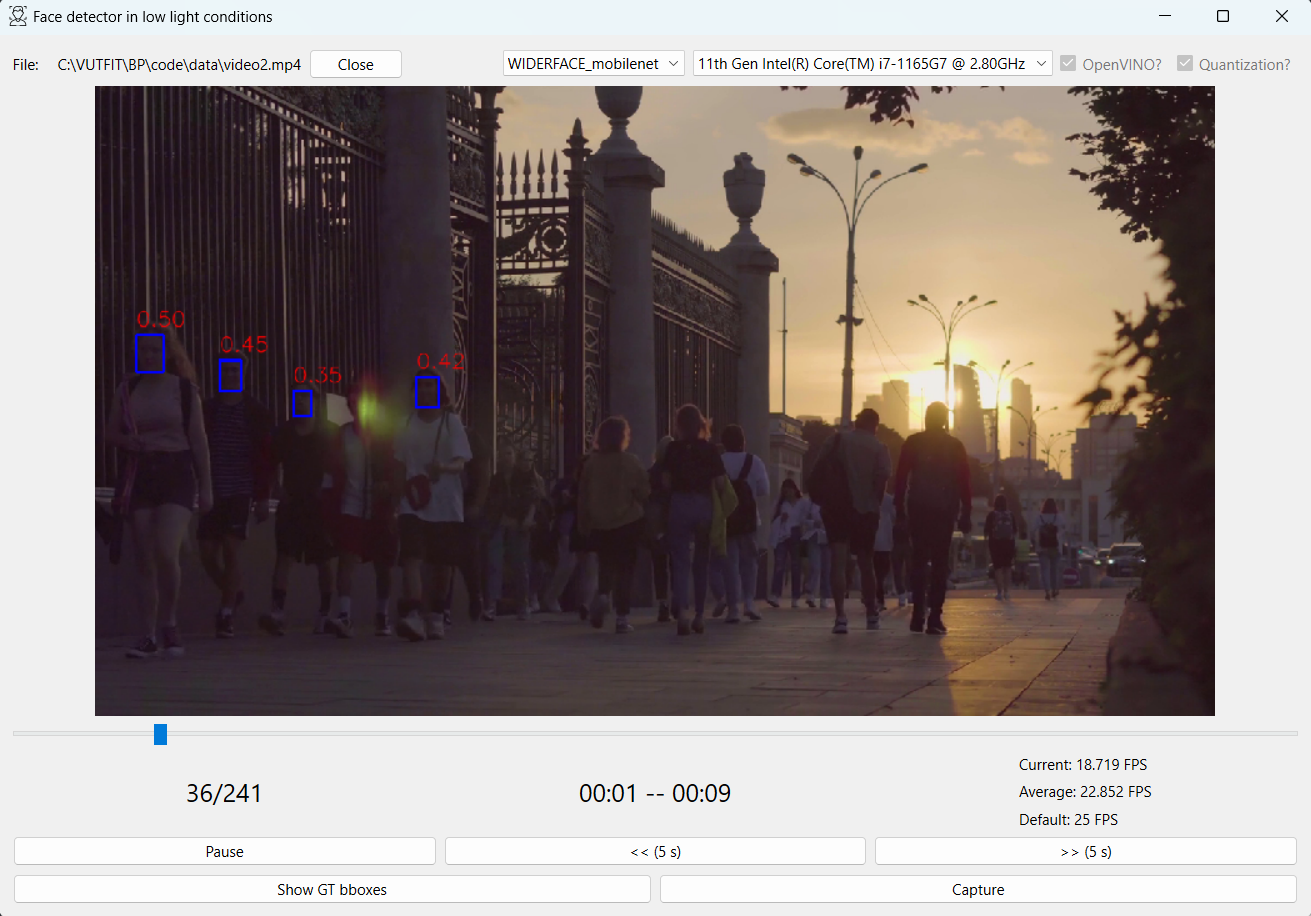
\includegraphics{obrazky-figures/gui.png}}
  \label{obrazek:gui}
  \caption{Aplikace pro detekci obličejů ve zhoršených světelných podmínkách}
  \end{center}
\end{figure}

\subsection*{Měřené metriky}
Při přehrávání videa nedochází pouze k detekci tváří, ale jsou zaznamenávány i metriky detekce. Mezi tyto metriky patří:

\begin{itemize}
  \item aktuální FPS,
  \item počet detekcí v aktuálním snímku,
  \item počet a polohy detekovaných obličejů ve formátu COCO.
\end{itemize}

\textbf{Aktuální FPS} jsou vypočítány pomocí doby uběhlé mezi začátkem detekce a zakreslením hraničních boxů kolem detekovaných tváří do snímku. 
\textbf{Počet detekcí} aplikace zaznamenává pro každý snímek zvlášť. Tyto dvě metriky jsou exportovány v csv souborech k dalšímu zpracování (viz sekce \ref{sekce:nastroje_pro_experimenty}).

Ke každému snímku je do souboru nazev\_videa\_output.txt zapsán \textbf{počet detekovaných obličejů a jejich souřadnice} v anotačním formátu COCO. Textový soubor odpovídá formátu, který používá dataset WIDER FACE. Formát COCO byl zvolen z toho důvodu, že stejný formát mají anotační soubory testovacích videí a je tak usnadněna práce s vyhodnocováním přesnosti detekce napříč snímky videa. Program, který pracuje s tímto výstupem je popsán v oddílu \ref{sekce:nastroje_pro_experimenty}.


\subsection*{Příprava videí}
K otestování schopností detektorů byly vybrány 2 testovací videa. Obě videa bylo třeba oanotovat, k čemuž byl použit webový nástroj CVAT\footnote{\url{https://www.cvat.ai}} (Computer Vision Anottation Tool). 
Tento program umožňuje ve zpracovávaném videu projít každý jeden snímek (frame) a nastavit v něm ohraničující boxy jednotlivých tváří. Tento úkon bylo nutno udělat ručně a výstup slouží jak \emph{ground truth} údaje pro validaci a porovnávání modelů mezi sebou. Formát výstupu je možné zvolit v několika tvarech, pro zpracovaná videa byl zvolen výstup podobný anotaci WIDER FACE datasetu (číslo snímku, počet obličejů ve snímku, COCO souřadnice). Konkrétní vybraná videa jsou popsána v další kapitole. 

\subsection*{Detekce}
Detekce, správa ovládání a zápis statistických informací probíhá v aplikaci v separátním vláknu. Vlákno je vytvořeno pomocí PyQt6 knihovních tříd QThreadPool a QRunnable. Pomocí PyQt6 signálů jsou mezi hlavním vláknem aplikace a detekčním vláknem předávány informace o snímkové frekvenci a aktuálním snímku s využitím slotových funkcí v rámci hlavního aplikačního vlákna. Další funkcionalita detekčního vlákna je zápis výstupních informací do csv souborů a předávání snímku s detekovanými obličeji pro vykreslení v hlavním vlákně.

Nastavení druhu používaného modelu, výběr zda využít jeho akcelerovanou nebo případně kvatovanou verzi je v gesci hlavního vlákna. Modely se nastavují jako globální proměnné, takže jsou dostupné ve všech funkcích a třídách aplikace.

O detekci se starají dvě hlavní funkce, obě jsou globální. Funkce \texttt{detect\_faces} je funkce pro detekci OpenVINO verzí modelu, podobně pojmenovaná funkce \texttt{detect\_faces\_tf} pak spouští detekci na TensorFlow variantě modelu. Která z funkcí bude využita definuje uživatelem dané nastavení v horním ovládacím řádku aplikace. Toto nastavení nelze již během zpracovávání videa měnit. Pro nastavení jiného modelu je třeba video uzavřít, změnit nastavení a video soubor znovu načíst.

Detekováné tváře, respektive jejich ohraničující body a důvěra modelu ve správnost detekce (\emph{confidence}), jsou hlavním výstupem obou vvýše zmíněných funkcí. Na vykreslení obdélníků do snímku dbá funkce \texttt{apply\_bboxes}, jenž zároveň vrací souřadnice v COCO formátu pro uložení do výstupního souboru k dalšímu zpracování.

Pokud je k pouštěnému videu dostupný anotační soubor (pojmenovaný formou nazev\_videa\_gt.txt) z aplikace CVAT, umí program ukazovat zelenou barvou \emph{ground truth} boxy. Tato utilita se zapíná tlačítkem \uv{Show GT boxes} a může posloužit k vizuální kontrole detekce uživatelem.

\section{Nástroje pro experimenty}
\label{sekce:nastroje_pro_experimenty}
Nástroje pro porovnávání modelů a experimenty s nimi jsou potřeba proto, aby bylo možné zhodnotit rozdíly mezi akcelerovaným a neakcelerovaným řešením a porovnat implementované detektory s existujícími.

% přepsat TODO
Tato část popisuje skripty pro zpracování výsledků detektorů obličejů a způsoby jejich porovnávání pro možnosti experimentů v další kapitole. Je zde vylíčeno jak se každá měřená metrika vyhodnocuje a jak vypadají výstupy experimentačních programů.
%konec přepsat

\subsection*{Evaluace}
Modely jsou v této práci porovnávány ve dvou kategoriích: \textbf{detekce ve videu} a \textbf{detekce v obrázcích z validačního datasetu}. K validaci je nutno stanovit některé pojmy a rovnice podle nichž dochází k vyhodnocování. Tyto měřící metody vycházejí z \cite{detekceMetriky}. Základním prvkem je výpočet \textbf{IoU} (průnik nad sjednocením, anglicky \emph{Intersection over Union}). IoU udává poměr průniku plochy detekovaného obličeje s plochou \emph{ground truth} ohraničujícího boxu a sjednocení těchto ploch. Ukázka výpočtu viz obrázek \ref{obrazek:iou}.

\begin{figure}[H] % TODO
  \begin{center}
      \scalebox{0.54}{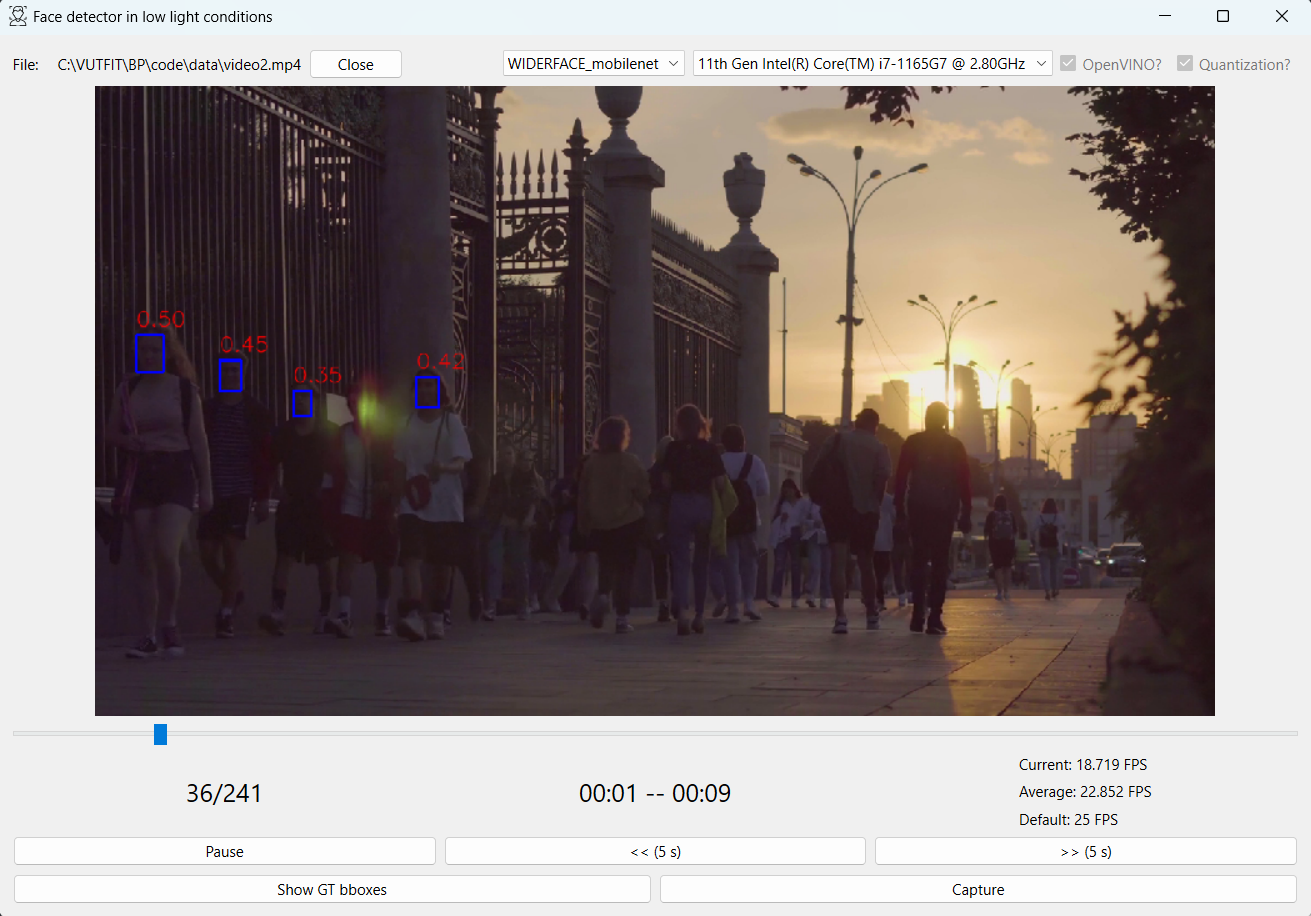
\includegraphics{obrazky-figures/gui.png}}
  \label{obrazek:iou}
  \caption{Výpočet IoU}
  \end{center}
\end{figure}

Hodnota IoU pak slouží k určení, zda byl překonán práh $t$ pro to, aby se dala detekce považovat za úspěšnou ($IoU \ge t$). Detekce tak může dopadnout jedním z následujících 4 způsobů:

\begin{itemize}
  \item True Positive (TP) -- správná detekce \emph{ground truth} boxu,
  \item False Positive (FP) -- detekce objektu tam, kde ve skutečnosti není,
  \item False Negative (FN) -- objekt nebyl detektorem detekován, přestože se zde nachází,
  \item True Negative (TN) -- objekt správně nebyl detekován.
\end{itemize}

Z těchto dat pak vychází 2 metriky, které se používají k měření úspěšnosti detekce. Přesnost detekce - poměr správných detekcí ke všem detekcím (dále jako \emph{precision}) a poměr správných detekcí ke všem \emph{ground truth} boxům (dále jako \emph{recall}). Tyto dvě čísla jsou vypočítána pomocí následujících rovnic:

\begin{equation}
  precision = \frac{TP}{TP + FP}
\end{equation}

\begin{equation}
  recall = \frac{TP}{TP + FN}
\end{equation}

\noindent Hodnoty obou metrik se nejčastěji vyjadřují v procentech.


\subsection*{Experimenty s videii}
Pro detekci ve videu slouží vytvořená GUI aplikace zaznamenávající data do csv souborů. Mezi hodnocené metriky patří:

\begin{itemize}
  \item průměrné FPS,
  \item průměrná přesnost detekce (\emph{precision}) v rámci jednotlivých snímků (framů),
  \item průměrná hodnota IoU mezi snímky.
\end{itemize}

Pro měření přesnosti a hodnoty IoU slouží skript zpracovávající výstupní soubor se souřadnicemi detekovaných obličejů. Průměrná hodnota FPS je pak vyčtena z grafu, který vytváří skript pro vizualizaci počtu FPS a počtu detekcí napříč snímky (ukázka viz obrázek). %TODO

Výpočet průměrné přesnosti je zpracován jako 11 bodová interpolace \cite{interpolace} \emph{precision} $\times$ \emph{recall} křivky (PR křivka). Tato křivka je tvořena z hodnot \emph{recall} na ose x a hodnot \emph{precision} na ose y. Hodnoty jsou zde vypočítány pomocí kumulativního součtu jednotlivých detekcí obličejů v obrázku, viz následující rovnice:

\begin{equation}
  precision_k = \frac{\sum_{i=0}^{k} TP}{\sum_{i=0}^{k} TP + \sum_{i=0}^{k} FP}
\end{equation}

\begin{equation}
  recall_k = \frac{\sum_{i=0}^{k} TP}{\sum_{i=0}^{k} TP + \sum_{i=0}^{k} FN}
\end{equation}

Tabulka \ref{tabulka:prkrivka} ukazuje příklad výpočtu hodnot \emph{precision} a \emph{recall} pro vytvoření křivky na obrázku s 6 obličeji (celkový počet \emph{ground truth} boxů je tak roven 6). Na obrázku \ref{obrazek:prkrivka} jsou tyto hodnoty přeneseny do grafu a je vykreslena spojovací křivka. Do pole hodnot pro vykreslení se navíc přidává bod na souřadnicích $[0, 1]$ aby byla křivka kompletní pro další výpočet.

\begin{table}[H]
  \begin{tabular}{|c|c|c|c|c|}
  \hline
  \rowcolor[HTML]{E0DBDB} 
  \textbf{Výsledek detekce} & \textbf{K. součet TP} & \textbf{K. součet FP} & \textbf{Precision} & \textbf{Recall} \\ \hline
  TP         & {\color[HTML]{3531FF} 1} & {\color[HTML]{FE0000} 0} & {\color[HTML]{3531FF} 1}/({\color[HTML]{3531FF} 1}+{\color[HTML]{FE0000} 0}) = 1 & {\color[HTML]{3531FF} 1}/6 = 0,166     \\ \hline
  FP    & 1   & 1     & 1/(1+1) = 0,5    & 1/6 = 0,166 \\ \hline
  TP   & 2    & 1   & 2/(2+1) = 0,66   & 2/6 = 0,33      \\ \hline
  TP    & 3    & 1   & 3/(3+1) = 0,75     & 3/6 = 0,5       \\ \hline
  FP   & 3     & 2     & 3/(3+2) = 0,6     & 3/6 = 0,5       \\ \hline
  TP  & 4    & 2   & 4/(4+2) = 0,66  & 4/6 = 0,66    \\ \hline
  \end{tabular}
  \label{tabulka:prkrivka}
  \caption{Příklad výpočtu \emph{precision} a \emph{recall} pro 11 bodovou interpolaci}
\end{table}

\begin{figure}[H] 
  \begin{center}
      \scalebox{0.8}{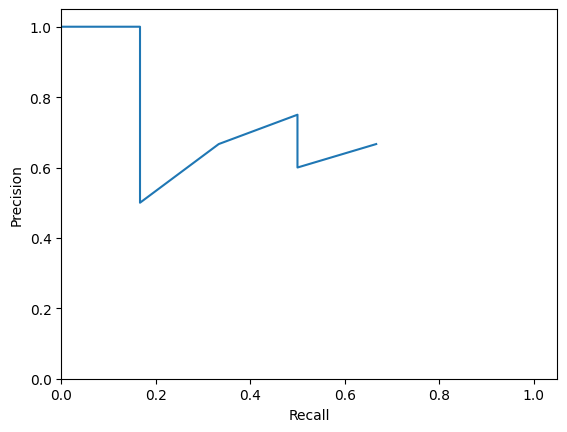
\includegraphics{obrazky-figures/prkrivka.png}}
  \label{obrazek:prkrivka}
  \caption{Graf PR přivky z příkladu z tabulky \ref{tabulka:prkrivka}}
  \end{center}
\end{figure}

Výsledká průměrná přesnost je vypočítána jako plocha pod křivkou. Tuto plochu můžeme vypočítat pomocí zmíněné 11 bodové interpolace. Tato metoda byla představena v roce 2007 v rámci detekční soutěže PASCAL VOC. Interpolace je prováděna na ose x (\emph{recall}) v bodech 0 až 1 s krokem 0,1 a jsou interpolovány hodnoty \emph{precision}, které v daném bodě odpovídají \textbf{nejvyšší hodnotě napravo}. Pro náš příklad by 11 interpolace vypadala tak, jak ukazuje graf na obrázku \ref{obrazek:interpolace}.

\begin{figure}[H] 
  \begin{center}
      \scalebox{0.8}{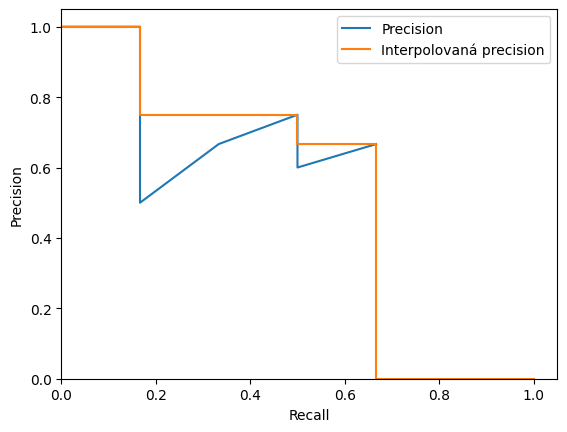
\includegraphics{obrazky-figures/interpolace.png}}
  \label{obrazek:interpolace}
  \caption{Graf interpolované přesnosti z příkladu}
  \end{center}
\end{figure}

\noindent Finální výpočet přesnosti pak vypadá následovně \cite{interpolace, detekceMetriky} (P = \emph{precision}, R = \emph{recall}):

\begin{equation}
  AP_{11} = \frac{1}{11} * \sum_{R \in \{0;0,1;...;0,9;1\}} P_{interpolovane} (R)
\end{equation}

Pro názorný příklad jsou interpolované hodnoty H rovny [1, 1, 0,75, 0,75, 0,75, 0,6666, 0,6666, 0, 0]. Výsledná přesnost tak je $AP = \frac{1}{11} * \sum H$ což se rovná cca 50,756 \%.

\subsection*{Experimenty s datasetem}
K měření úspěšnosti detekce v datasetu je využit validační dataset popsaný dále v sekci \ref{sekce:podklady}. Skripty měřící \emph{precision} a \emph{recall} umožňují nastavit model a zařízení na nichž se bude měřit. Evaluace je pak prováděna pomocí COCO evaluace\footnote{\url{https://cocodataset.org/\#detection-eval}}. 

COCO evaluace detekčních modelů počítá přesnost detekce s různými prahy $t$ pro hodnotu IoU. V experimentech v kapitole \ref{kapitola:experimenty} jsou naměřené hodnoty \emph{precision} pro tyto prahy:

\begin{enumerate}
  \item průměr mezi 0,5 až 0,95 s krokem 0,05
  \item 0,5
  \item 0,75
\end{enumerate}

\noindent Hodnota \emph{recall} se pak počítá pro:

\begin{enumerate}
  \item 1 detekci na 1 obrázek,
  \item 10 detekcí na 1 obrázek,
  \item 100 detekcí na 1 obrázek.
\end{enumerate}
 

%%%%%%%%%%%%%%%%%%%%%%%%%%%%%%%%%%%%%%%%%%%%%%%%%%%%%%%%%
%       KAPITOLA Experimenty
%%%%%%%%%%%%%%%%%%%%%%%%%%%%%%%%%%%%%%%%%%%%%%%%%%%%%%%%%
\chapter{Experimenty}
\label{kapitola:experimenty}

\section{Podklady}
\label{sekce:podklady}


Mezi data, která jsou hodnocena za účelem srovnání detekčních sítí, patří nejen data získaná z GUI aplikace, ale také výsledky evaluace modelů na validačním datasetu. Jako validační dataset byla vybrána část WIDER FACE datasetu určená k validaci s některými úpravami:
\begin{itemize}
  \item odebrání snímků s více než 100 obličeji,
  \item augmentace snímků, tak aby spadaly do kategorii zhoršených světelných podmínek.
\end{itemize}

\section{Porovnání akcelerovaného a normálního řešení}


\section{Detekce s a bez Mirnetu}

\section{Porovnání s YOLOFacev7}

\section{Porovnání s Viola--Jones}

\section{Porovnání s MTCNN}

%%%%%%%%%%%%%%%%%%%%%%%%%%%%%%%%%%%%%%%%%%%%%%%%%%%%%%%%%
%       KAPITOLA ZÁVĚR
%%%%%%%%%%%%%%%%%%%%%%%%%%%%%%%%%%%%%%%%%%%%%%%%%%%%%%%%%
\chapter{Závěr}
\label{kapitola:zaver}
V~rámci tohoto textu byla představena problematika detekce obličejů v~reálných podmínkách, dále byly popsány problémy omezující detekci a~klasické algoritmy detekce obličejů. V~samostatných kapitolách a~sekcích byly popsány neuronové sítě (obecně, konvoluční) a~algortimy pro detekci založené na neuronových sítích. Dále pak existující komerční a~nekomerční řešení, systémy detekce a možnosti akcelerace neuronových sítí specializovaným hardawarem.

V~této práci bude pokračováno návrhem neuronové sítě pro detekci ve špatných světelných podmínkách, návrhem Python aplikace, její implementací a provedením experimentů s~vytvořeným řešením a existujícími řešeními.